% ..............................................................................
% "KI in der Onkologie" -- Andreas Maier, MSD Senso-Abend (München, 11.06.2026).
% Deutsche Variante (Branch de-msd-senso) der "What next in medical AI?"-Folien
% mit zwei zusätzlichen Folien nach dem Bayerischen Basismodell zur
% multimodalen Datenintegration und Hypothesengenerierung am Beispiel
% der PRAEGNANT-Studie.
% ------------------------------------------------------------------------------
\documentclass[final]{beamer}

% Sneak ngerman + main=ngerman into babel BEFORE the FAU theme loads
% babel with english.  Once the theme later does \RequirePackage[english]{babel}
% the english option is already in the queue, so no option clash, and
% ngerman is the active main language.
\PassOptionsToPackage{main=ngerman,ngerman,english}{babel}

\usepackage[institute=Tech,
            aspectratio=169,
            fontsize=11,
            fontbaselineskip=13,
            scale=1.,
            InsertTotalFoot
           ]{styles/beamerthemefau}

\usepackage[utf8]{inputenc}
\usepackage[T1]{fontenc}
\usepackage{graphicx}
\usepackage{textcomp}
\usetikzlibrary{positioning,arrows.meta,shadows}

\graphicspath{{figures/}}

% ----------------------------------------------------------------------------------------
% Titel-Metadaten
% ----------------------------------------------------------------------------------------
\title[KI in der Onkologie]{KI in der Onkologie}
\subtitle{Neueste Fortschritte und zukünftige Anwendungen}
\author[A.~Maier]{Andreas Maier}
\institute[FAU]{Friedrich-Alexander-Universität Erlangen-Nürnberg}
\date{11.~Juni 2026, München}

% ================================================
% Hauptdokument
% ------------------------------------------------
\begin{document}

% --------------------------------------------------------------------------
% Folie 1 - Titel
% --------------------------------------------------------------------------
\begin{frame}[t,titleimage]{-}
\titlepage%
\end{frame}

% --------------------------------------------------------------------------
% Folie 2 - Übersicht
% --------------------------------------------------------------------------
\begin{frame}[t]{Übersicht}
\begin{itemize}
  \item Was ist Deep Learning?
  \item Was ist agentische KI?
  \item Wie geht es weiter?
\end{itemize}
\end{frame}

% --------------------------------------------------------------------------
% Folie 3 - Abschnittstrenner
% --------------------------------------------------------------------------
\begin{frame}[t,title]{-}
Was ist Deep Learning?
\end{frame}

% --------------------------------------------------------------------------
% Folie 4 - Deep Learning (4 Unterfolien)
% --------------------------------------------------------------------------
\begin{frame}[t]{Deep Learning}{Spracherkennung}
\begin{itemize}
  \item Revolutioniert Mustererkennung und KI seit über 10~Jahren.
\end{itemize}
\vspace{0.2em}
\begin{center}
  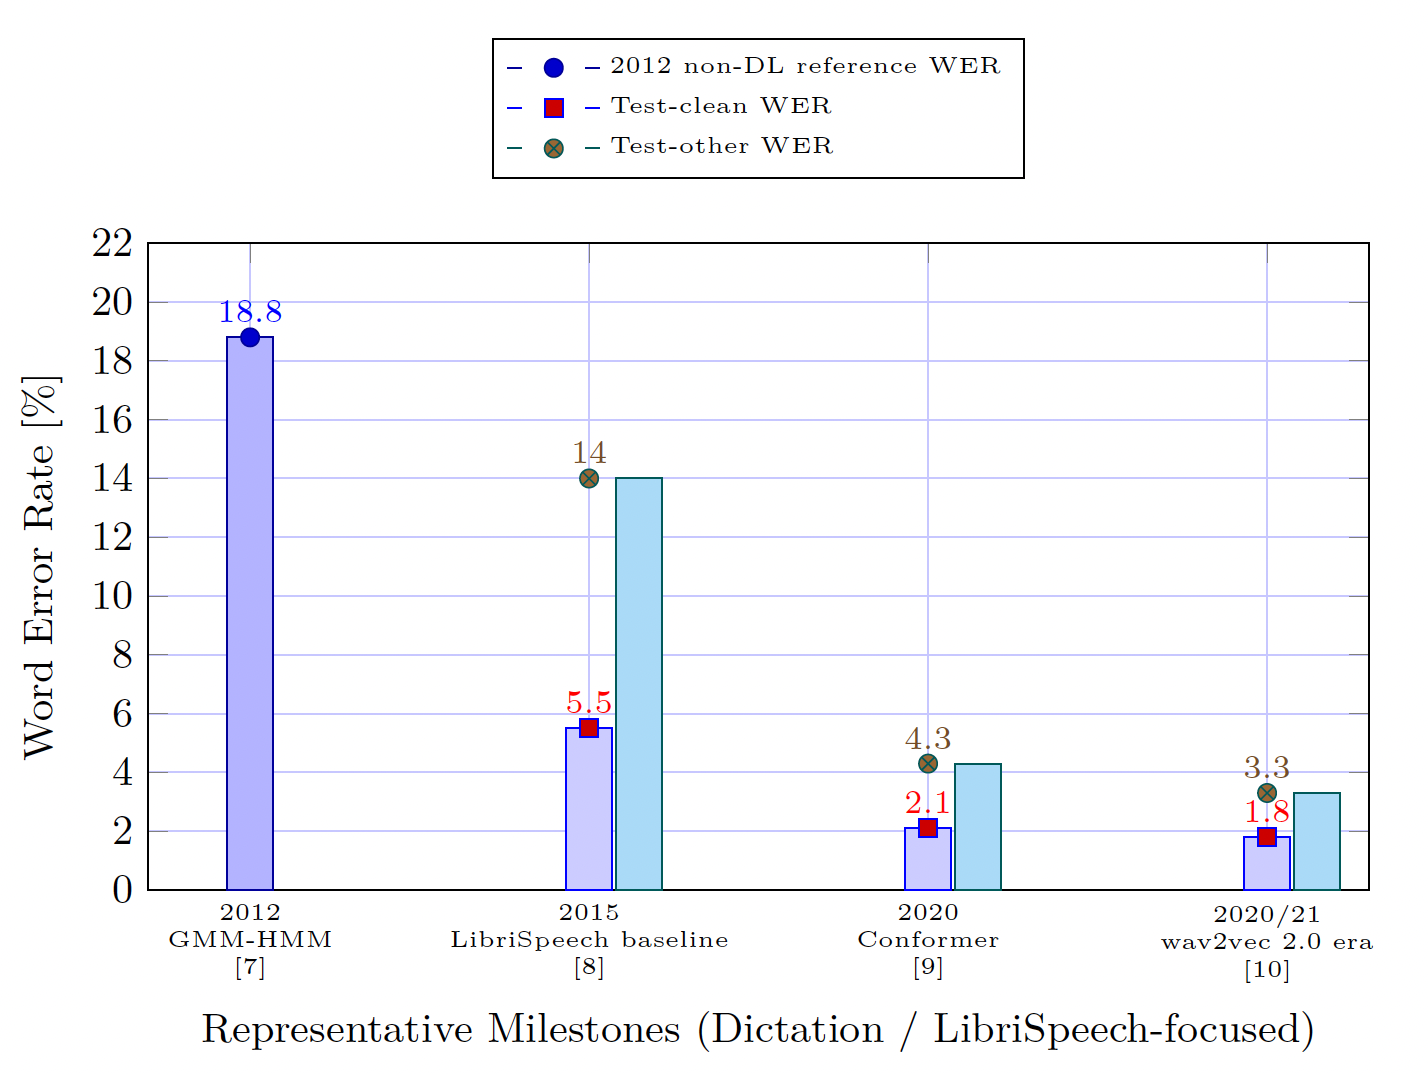
\includegraphics[height=.6\textheight]{img_03_03.png}
\end{center}
\end{frame}

\begin{frame}[t]{Deep Learning}{Bildklassifikation}
\begin{center}
  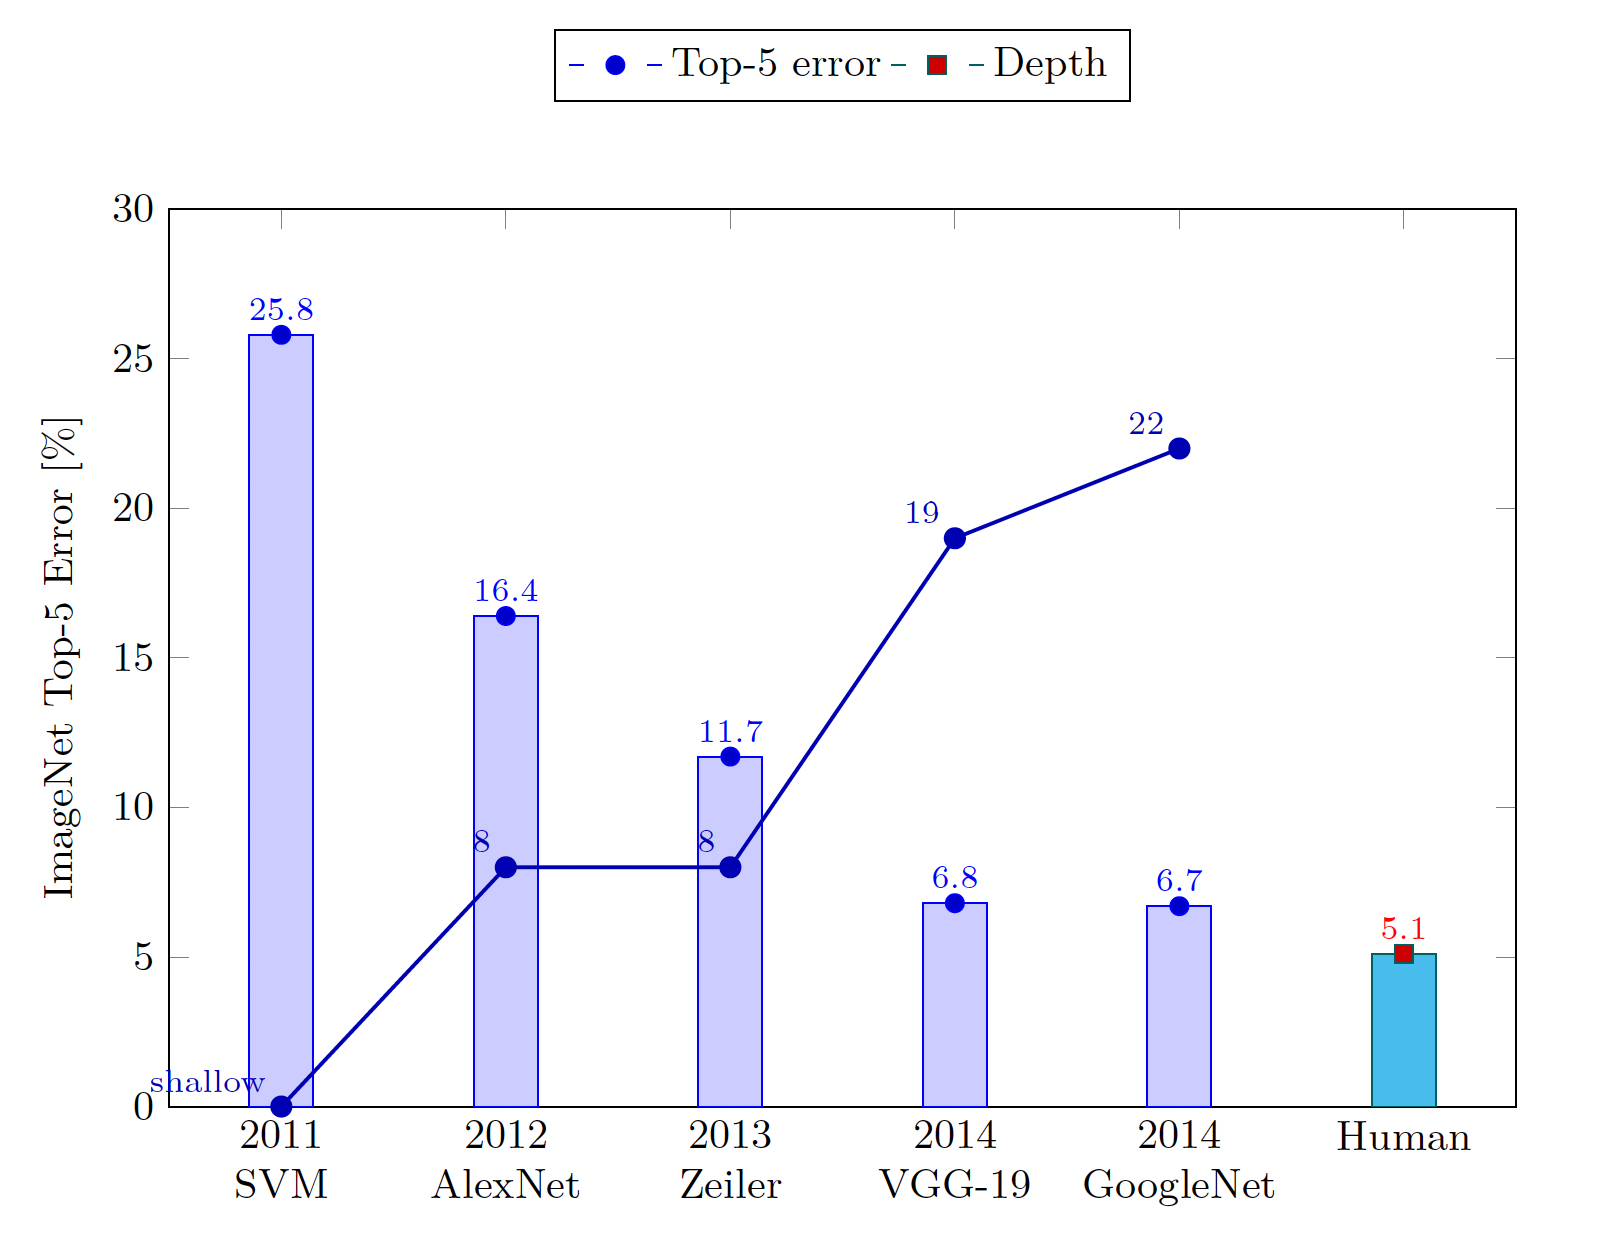
\includegraphics[height=.7\textheight]{img_03_04.png}
\end{center}
\end{frame}

\begin{frame}[t]{Deep Learning}{Spielen lernen}
\begin{center}
  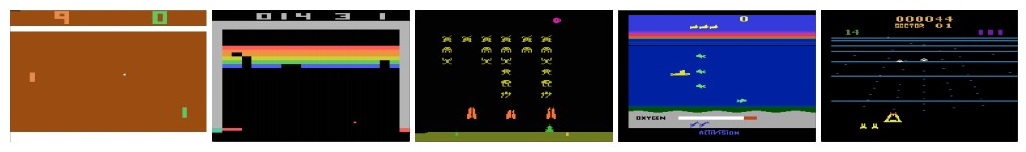
\includegraphics[width=.95\textwidth]{img_03_05.png}\\[0.2em]
  {\footnotesize [Mnih 2013]}
\end{center}
\vspace{0.3em}
\begin{itemize}\itemsep=0.15em
  \item Deep Q-Networks lernen Atari-Spiele allein aus den Pixeln.
  \item Ein Agent, viele Spiele -- in mehreren Titeln übermenschlich.
\end{itemize}
\pause
\vspace{0.4em}
\begin{columns}[c]
  \begin{column}{0.45\textwidth}
    \centering
    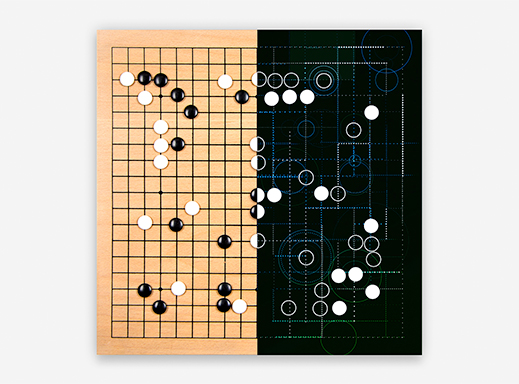
\includegraphics[height=.30\textheight]{img_03_06.jpg}\\
    {\footnotesize AlphaGo (DeepMind, 2016)}
  \end{column}
  \begin{column}{0.5\textwidth}
    \begin{itemize}\itemsep=0.15em
      \item Selbstspiel $+$ Monte-Carlo-Baumsuche.
      \item Schlägt Weltmeister Lee Sedol mit 4--1.
    \end{itemize}
  \end{column}
\end{columns}
\end{frame}

% --------------------------------------------------------------------------
% Folie 5 - Generative KI (4 Unterfolien)
% --------------------------------------------------------------------------
\begin{frame}[t]{Generative KI}{Originalbild}
\begin{center}
  
\includegraphics[height=.75\textheight]{img_04_01.jpg}
\end{center}
\end{frame}

\begin{frame}[t]{Generative KI}{Bildbeschreibung}
\begin{columns}[T]
  \begin{column}{0.32\textwidth}
    \centering
    
\includegraphics[height=.75\textheight]{img_04_01.jpg}
  \end{column}
  \begin{column}{0.66\textwidth}
    \vspace{0.4em}
    \normalsize\itshape
    \glqq Ein athletisch gebauter Mann mit ernstem Gesichtsausdruck steht
    in einem gut beleuchteten Raum mit Holzdecke. Er trägt ein blaues
    T-Shirt mit dem Aufdruck \glq SAVE THE CHUBBY UNICORNS\grq{} und
    dem Bild eines Nashorns. Der Mann macht ein Selfie mit einem
    modernen Smartphone und fotografiert sein Spiegelbild. Im
    Hintergrund sind Trainingsgeräte zu sehen, darunter Hanteln und
    ein Hantelständer. Außerdem hängt ein Kronleuchter mit
    eigenwilligem Design von der Decke und beleuchtet den Raum.\grqq
  \end{column}
\end{columns}
\end{frame}

\begin{frame}[t]{Generative KI}{Generiertes Bild}
\begin{center}
  
\includegraphics[height=.75\textheight]{img_04_04.jpg}
\end{center}
\end{frame}

\begin{frame}[t]{Generative KI}{Stilvarianten}
\begin{columns}[c]
  \begin{column}{0.5\textwidth}
    \centering
    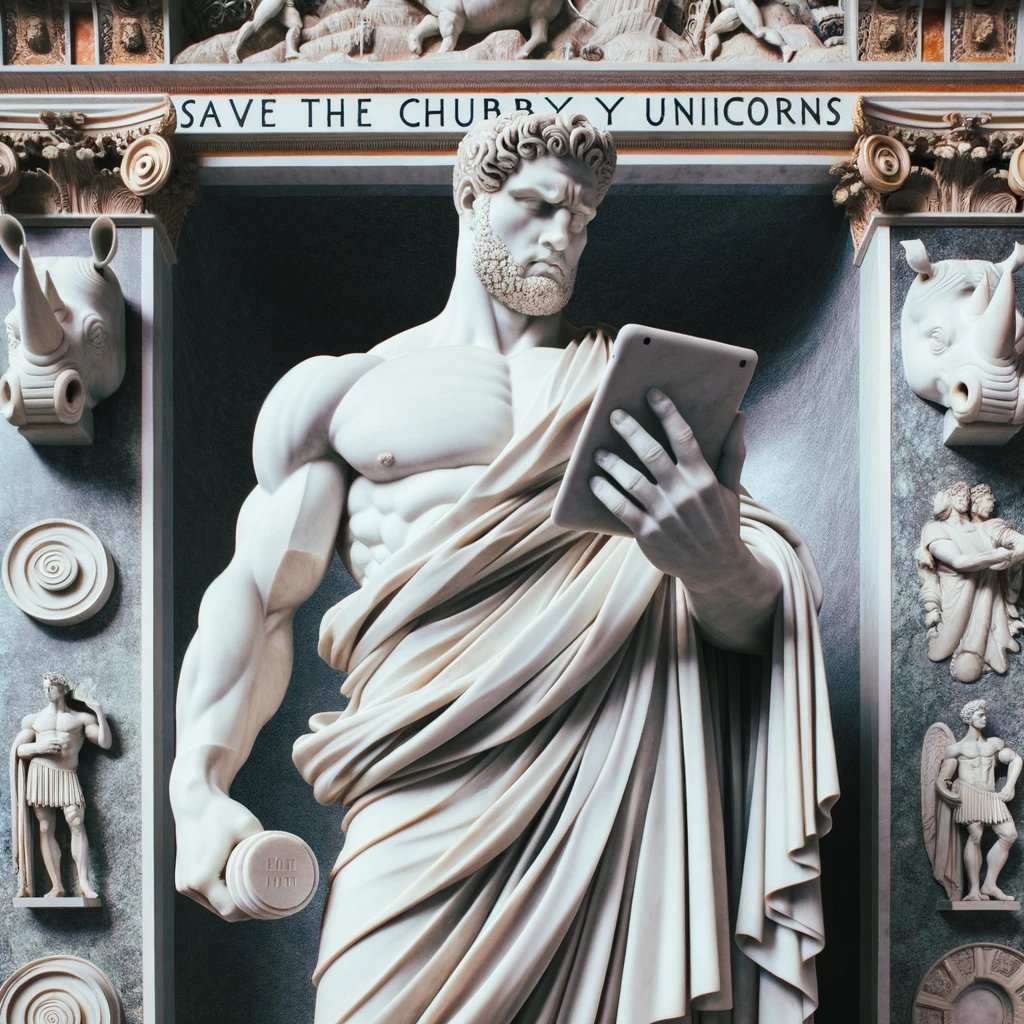
\includegraphics[height=.7\textheight]{img_04_06.jpg}
  \end{column}
  \begin{column}{0.5\textwidth}
    \centering
    \onslide<2->{
\includegraphics[height=.7\textheight]{img_04_05.jpg}}
  \end{column}
\end{columns}
\end{frame}

% --------------------------------------------------------------------------
% Folie 6 - Deep Learning in der Medizin (4 Unterfolien)
% --------------------------------------------------------------------------
\begin{frame}[t]{Deep Learning in der Medizin}{Von der Segmentierung zur Rekonstruktion}
\begin{columns}[c]
  \begin{column}{0.55\textwidth}
    \centering
    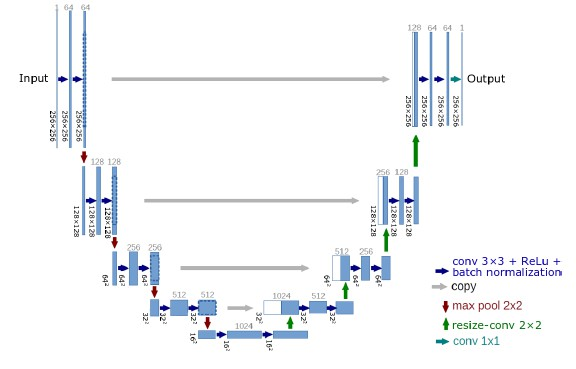
\includegraphics[height=.7\textheight]{img_05_01.jpg}
  \end{column}
  \begin{column}{0.45\textwidth}
    \centering
    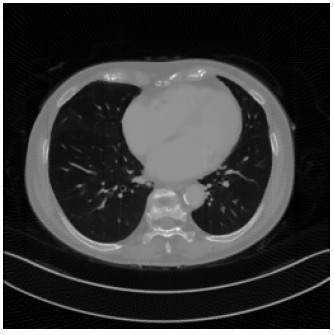
\includegraphics[height=.5\textheight]{img_05_02.jpg}
  \end{column}
\end{columns}
\end{frame}

\begin{frame}[t]{Deep Learning in der Medizin}{Bekannte Operatoren}
\vspace*{0.4em}
\begin{center}
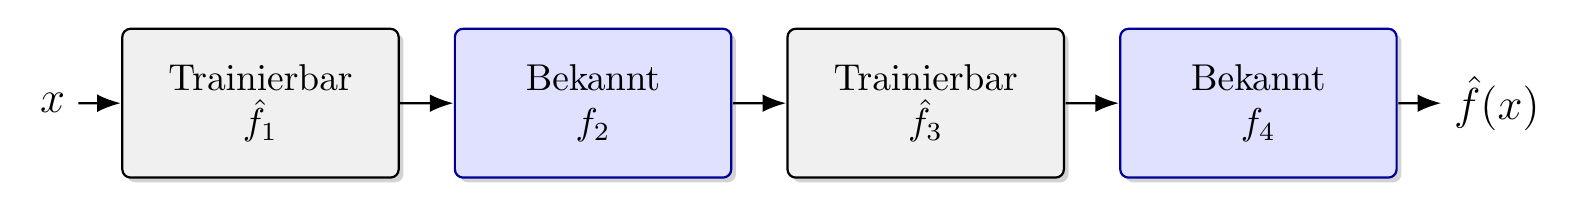
\begin{tikzpicture}[
    every node/.style={font=\normalsize},
    transform shape, scale=1.35,
    box/.style ={draw, rounded corners=3pt, minimum height=1.4cm,
                 minimum width=2.6cm, align=center, thick,
                 drop shadow={shadow xshift=0.6mm, shadow yshift=-0.6mm,
                              opacity=0.35}},
    train/.style={box, fill=gray!12},
    known/.style={box, fill=blue!12, draw=blue!60!black},
    arr/.style ={-{Latex[length=3mm]}, thick}
  ]
  \node                                 (in)  {\large $x$};
  \node[train, right=4mm of in]         (t1)  {Trainierbar\\$\hat f_1$};
  \node[known, right=5mm of t1]         (k1)  {Bekannt\\$f_2$};
  \node[train, right=5mm of k1]         (t2)  {Trainierbar\\$\hat f_3$};
  \node[known, right=5mm of t2]         (k2)  {Bekannt\\$f_4$};
  \node[right=4mm of k2]                (out) {\large $\hat f(x)$};
  \draw[arr] (in)  -- (t1);
  \draw[arr] (t1)  -- (k1);
  \draw[arr] (k1)  -- (t2);
  \draw[arr] (t2)  -- (k2);
  \draw[arr] (k2)  -- (out);
\end{tikzpicture}\\[0.5em]
{\small Kombination \emph{trainierbarer} Schichten mit deterministischen
Operatoren (Fourier-Transformation, Gradientenabstieg, Projektion, \dots).}
\end{center}
\pause
\vspace{0.5em}
\begin{block}{Theorem -- bekannte Operatoren verkleinern die Fehlerschranke}
Für $f=f_n\circ\dots\circ f_1$, approximiert durch
$\hat f=\hat f_n\circ\dots\circ \hat f_1$ mit Schichtfehlern
$\varepsilon_i$ und Lipschitz-Konstanten $\hat L_j$, gilt
\[
  \varepsilon(\hat f) \;\leq\;
  \sum_{i=1}^{n}\Bigl(\prod_{j=i+1}^{n}\hat L_j\Bigr)\,\varepsilon_i .
\]
Ersetzt man $\hat f_k$ durch den \emph{bekannten} Operator $f_k$, wird
$\varepsilon_k=0$ und die Schranke verbessert sich strikt.
\end{block}
\vspace{-0.3em}
\begin{center}\footnotesize
  Maier et al., \emph{Nature Machine Intelligence}, 2019.
\end{center}
\end{frame}

\begin{frame}[t]{Deep Learning in der Medizin}{Rekonstruktion}
\begin{columns}[c]
  \begin{column}{0.5\textwidth}
    \centering
    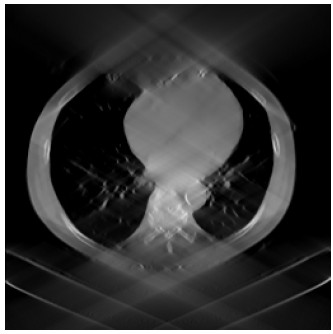
\includegraphics[height=.65\textheight]{img_05_03.jpg}\\[0.4em]
    \footnotesize Klassisch
  \end{column}
  \begin{column}{0.5\textwidth}
    \centering
    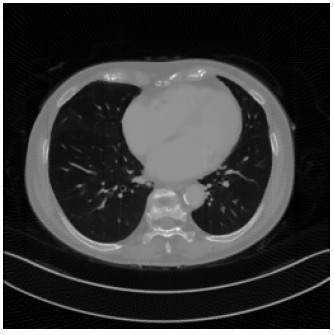
\includegraphics[height=.65\textheight]{img_05_02.jpg}\\[0.4em]
    \footnotesize Mit Deep Learning
  \end{column}
\end{columns}
\end{frame}

\begin{frame}[t]{Deep Learning in der Medizin}{MRT-Variational-Network}
\begin{center}
  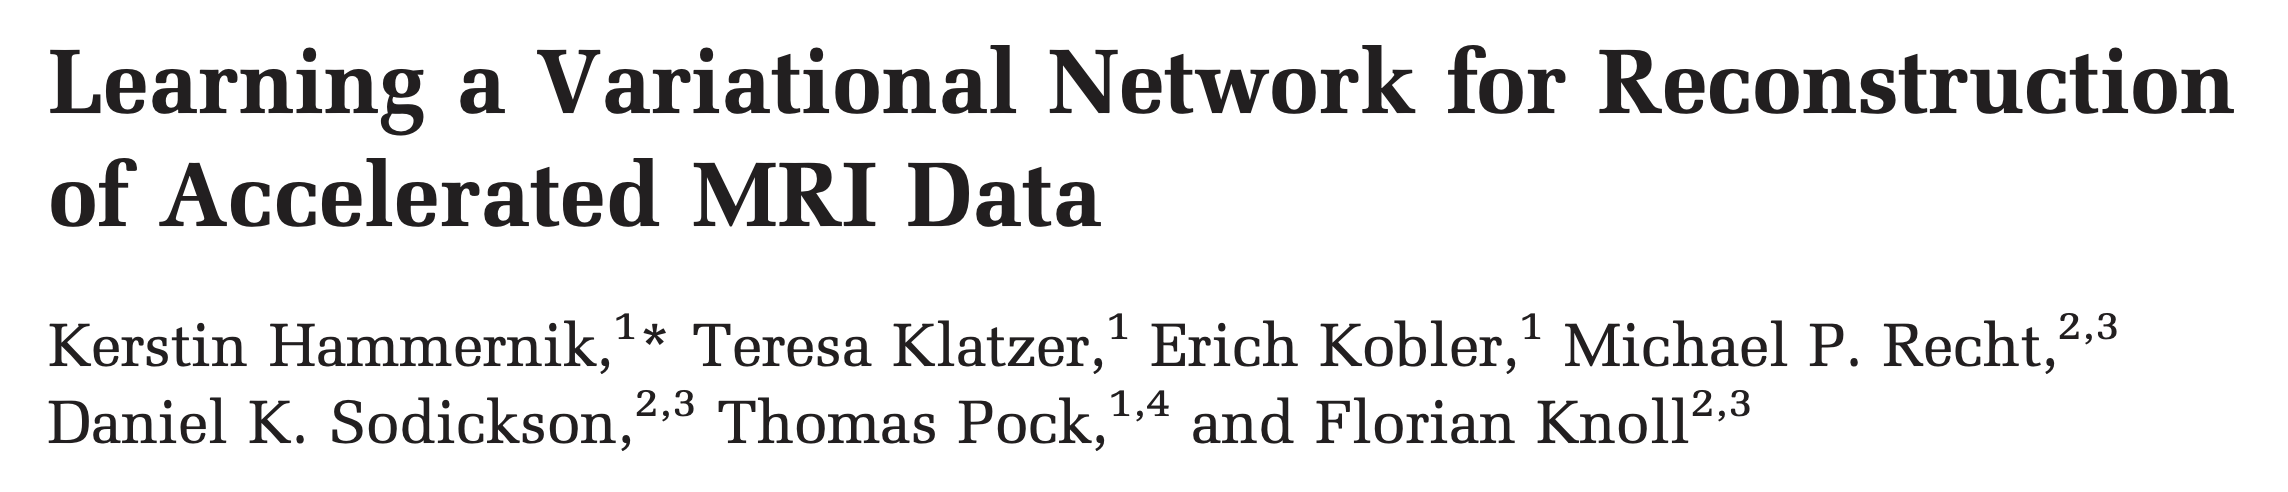
\includegraphics[width=.55\textwidth]{img_05_05.png}\\[0.5em]
  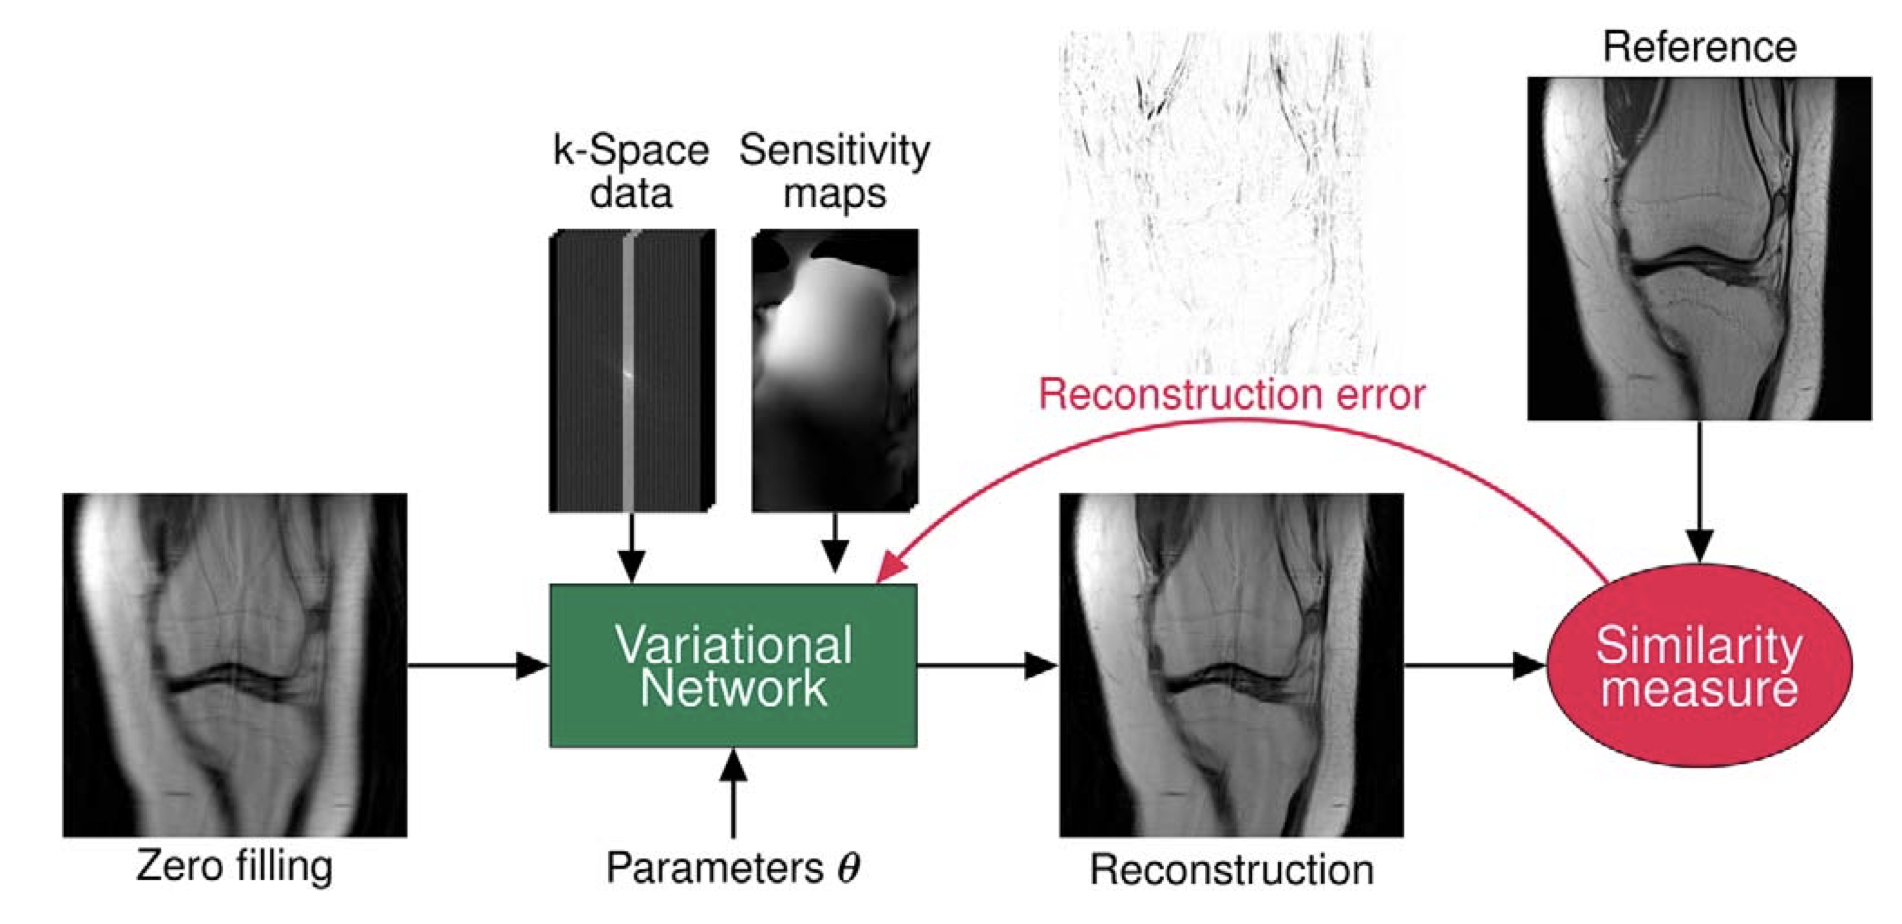
\includegraphics[width=.6\textwidth]{img_05_04.png}
\end{center}
\end{frame}

\begin{frame}[t]{Deep Learning in der Medizin}{Auszeichnung}
\begin{columns}[c]
  \begin{column}{0.35\textwidth}
    \centering
    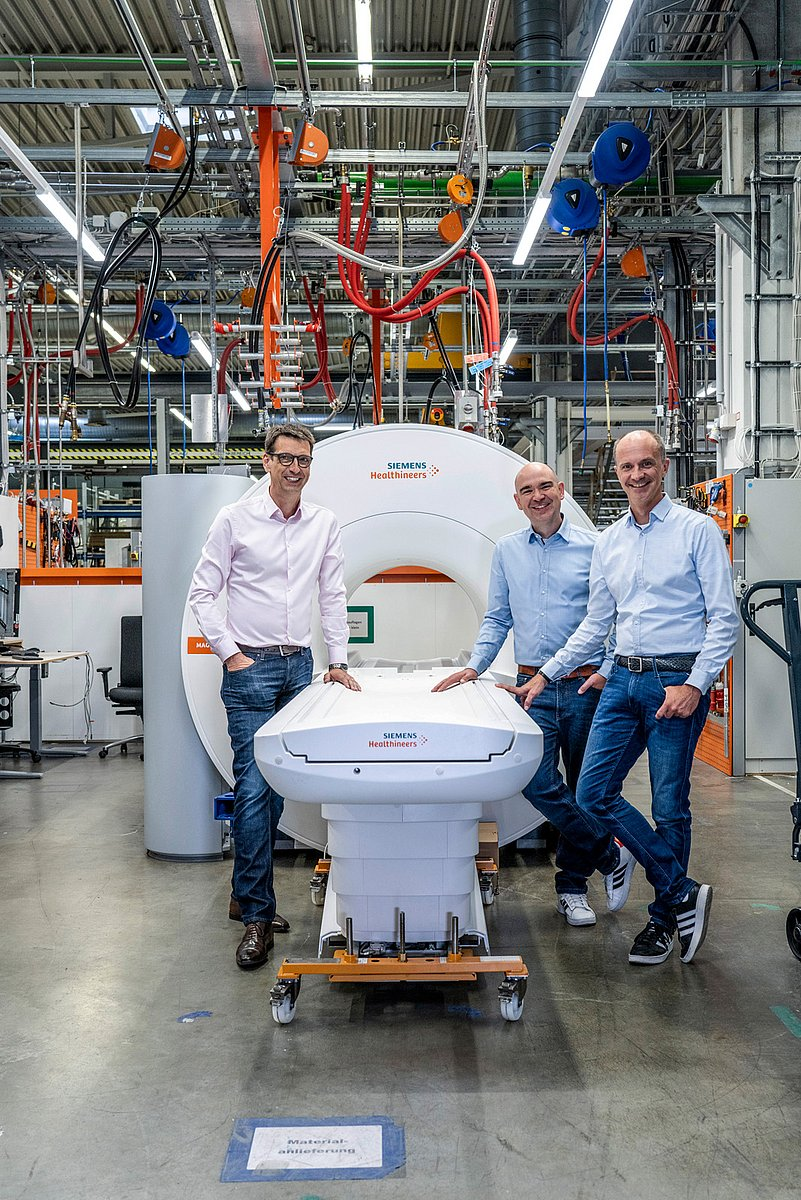
\includegraphics[height=.72\textheight,keepaspectratio]{siemens01.jpg}
  \end{column}
  \begin{column}{0.62\textwidth}
    \centering
    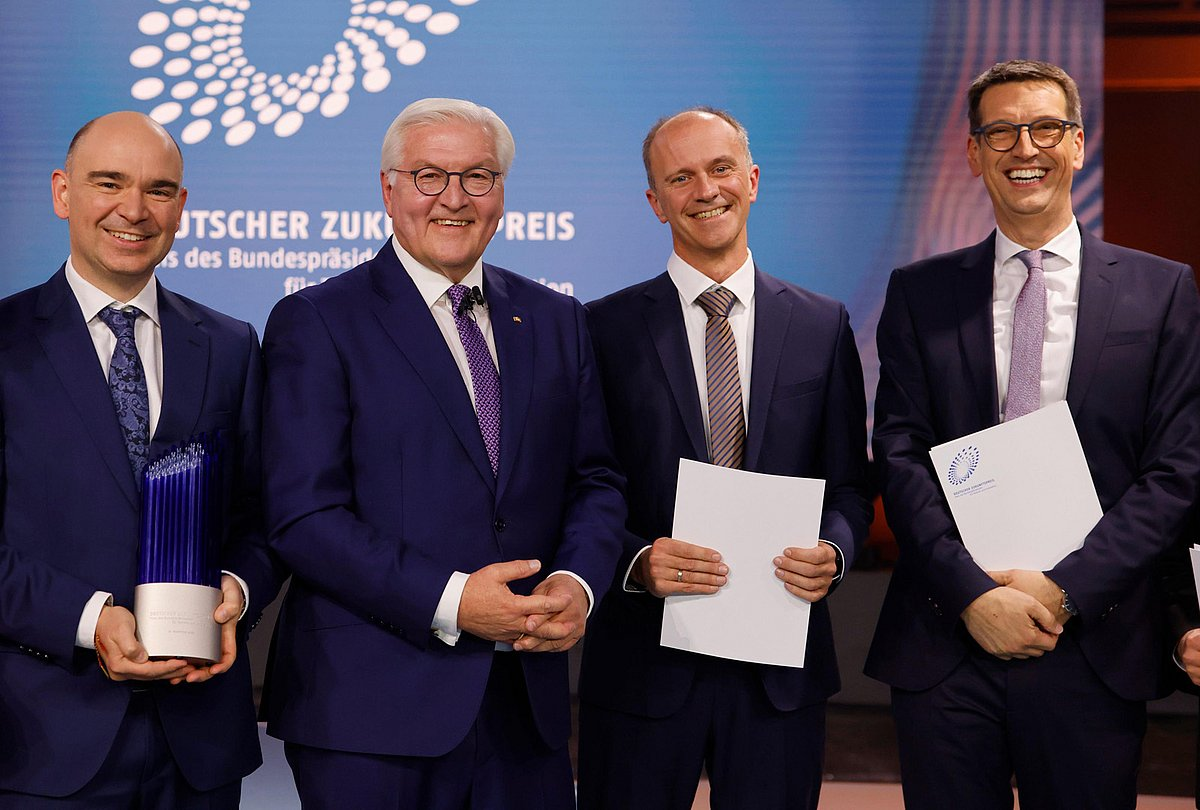
\includegraphics[width=\linewidth,height=.72\textheight,keepaspectratio]{siemens02.jpg}
  \end{column}
\end{columns}
\vspace{0.4em}
\begin{center}
  Deutscher Zukunftspreis -- Niederfeld-MRT, ermöglicht durch Deep Learning.
\end{center}
\end{frame}

% --------------------------------------------------------------------------
% Folie 7 - Abschnittstrenner
% --------------------------------------------------------------------------
\begin{frame}[t,title]{-}
Was ist agentische KI?
\end{frame}

% --------------------------------------------------------------------------
% Folie 8 - Was ist agentische KI? Einführung (3 Unterfolien)
% --------------------------------------------------------------------------
\begin{frame}[t]{Was ist agentische KI?}{Eine einfache Frage}
\vspace*{0.6em}
\begin{flushleft}
  {\Huge\itshape\glqq Wie fährt man ein Auto?\grqq}
\end{flushleft}
\vspace*{0.6em}
{\large\color{gray}\itshape Hat einige Sekunden nachgedacht\dots}
\vspace*{1.4em}
\begin{itemize}\large
  \item Ein klassischer Prompt an ein großes Sprachmodell.
  \item Nach einer kurzen \glqq Denkpause\grqq{} erscheint die Antwort
        als langer Fließtext.
  \item Keine Werkzeuge, keine Aktionen -- das Modell \emph{beschreibt}
        nur, wie man fährt.
\end{itemize}
\end{frame}

\begin{frame}[t]{Was ist agentische KI?}{Lange Textantwort eines LLMs}
\normalsize
Um ein Auto zu fahren, gehen Sie wie folgt vor:
\begin{itemize}\itemsep=0.3em
  \item \textbf{Einsteigen und einstellen:} \textbf{Sicherheitsgurt}
        anlegen, \textbf{Sitz} und \textbf{Spiegel} so einstellen, dass
        Sie die Straße gut überblicken.
  \item \textbf{Motor starten:} \textbf{Bremspedal} treten, Schlüssel
        drehen oder Startknopf drücken. Der Wählhebel muss auf
        \textbf{Park (P)} oder \textbf{Neutral (N)} stehen.
  \item \textbf{Gang einlegen:} Beim Automatikgetriebe Hebel auf
        \textbf{Drive (D)}; beim Schaltgetriebe \textbf{Kupplung}
        treten und den \textbf{1.~Gang} einlegen.
  \item \textbf{Handbremse lösen} und Fuß langsam von der Bremse
        nehmen. Sanft auf das \textbf{Gaspedal} treten, um anzufahren.
  \item \textbf{Lenken} Sie mit beiden Händen und beobachten Sie
        regelmäßig die \textbf{Spiegel}. Sicherheitsabstand zum
        vorausfahrenden Fahrzeug einhalten.
  \item \textbf{Zum Anhalten:} Gas wegnehmen, Bremse treten und das
        Fahrzeug vollständig zum Stehen bringen. In \textbf{Park}
        schalten und Handbremse anziehen, bevor der Motor
        ausgeschaltet wird.
\end{itemize}
\vspace{0.6em}
\begin{center}\itshape\color{gray}
Beachten Sie stets die Verkehrsregeln und passen Sie Ihre Fahrweise
an Straße und Wetter an.
\end{center}
\vspace{0.4em}
\hfill\textbf{$\Rightarrow$ Viele Worte, aber keine \emph{Aktion}.}\hfill\,
\end{frame}

\begin{frame}[t]{Was ist agentische KI?}{Vom Sprachmodell zum Agenten}
\begin{columns}[c]
  \begin{column}{0.48\textwidth}
    \centering
    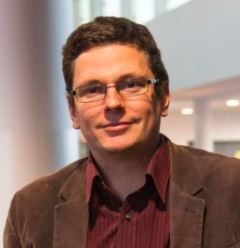
\includegraphics[height=.4\textheight]{img_07_03.jpg}\\[0.3em]
    \footnotesize Moritz Zaiss
  \end{column} \pause
  \begin{column}{0.48\textwidth}
    \centering
    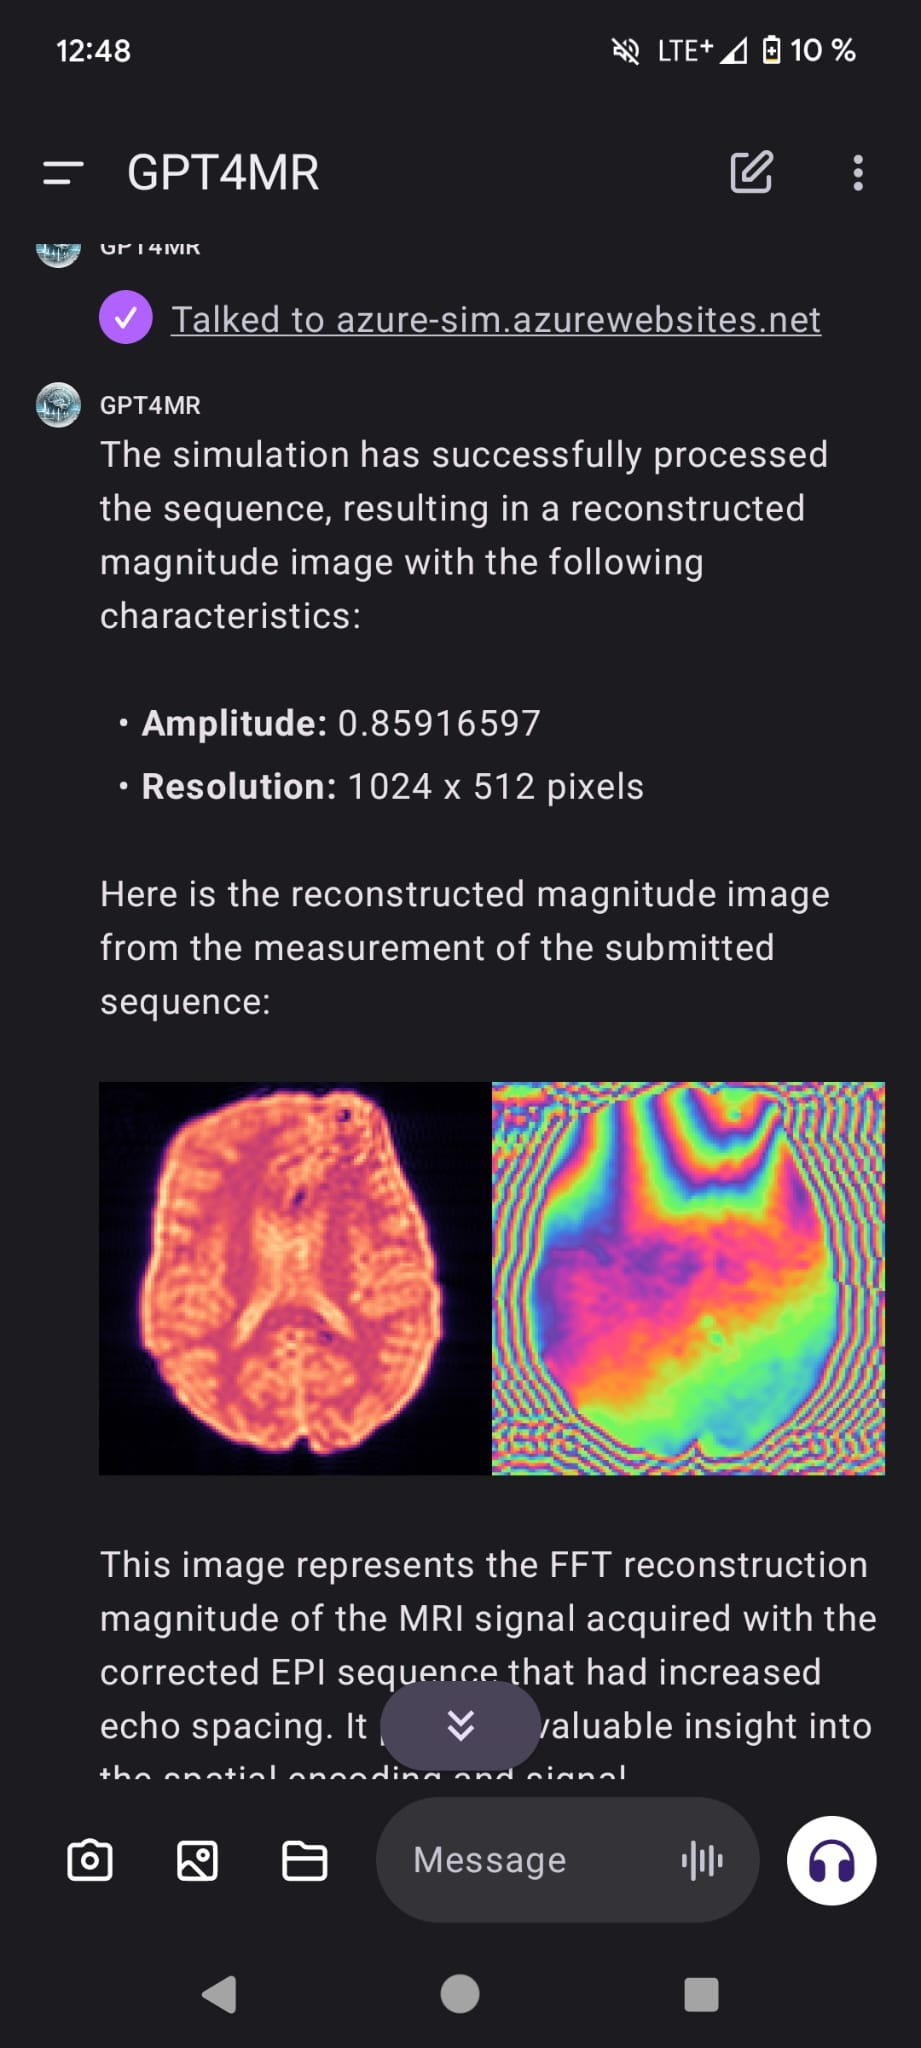
\includegraphics[height=.76\textheight,keepaspectratio]{img_07_01.png}
    \vspace{-0.5cm}
    \begin{center}
      {\footnotesize Zaiss et al., \emph{GPT4MR}, 2024.}
    \end{center}
  \end{column}
\end{columns}
\vspace{0.2em}
\end{frame}

% --------------------------------------------------------------------------
% Folie 9 - Spin-Echo-EPI: 3 Modellversuche (4 Unterfolien, animiert)
% --------------------------------------------------------------------------
\begin{frame}[t]{Was ist agentische KI?}{Aufgabe für die Modelle}
\vspace*{0.4em}
\begin{center}
  \begin{minipage}{.92\textwidth}
    \large\itshape
    \glqq Programmiere ein Spin-Echo-EPI (64$\times$64,
    fov\,=\,(0{,}2,\,0{,}2,\,0{,}08)\,m,
    TE\,=\,150\,ms)!\grqq
  \end{minipage}
\end{center}
\vspace*{0.6em}
\begin{itemize}\large\itemsep=0.3em
  \item \textbf{Spin-Echo-EPI} -- eine fortgeschrittene MRT-Sequenz
        für Diffusions- und funktionelle Bildgebung.
  \item Drei Modelle erhalten \emph{dieselbe} natürlichsprachliche
        Anweisung und müssen lauffähigen Python-Code erzeugen.
  \item Teilnehmer:
\end{itemize}
\vspace*{0.2em}
\begin{center}
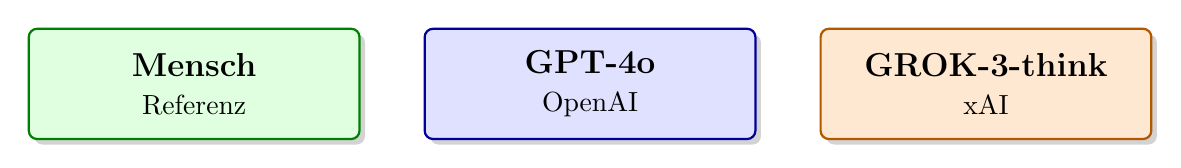
\begin{tikzpicture}[
    every node/.style={font=\large\bfseries},
    box/.style={draw, rounded corners=3pt, thick,
                minimum height=1.4cm, minimum width=4.2cm,
                text width=3.8cm, align=center,
                drop shadow={shadow xshift=0.7mm, shadow yshift=-0.7mm,
                             opacity=0.35}}
  ]
  \node[box, fill=green!12, draw=green!50!black] (h)               {Mensch\\\normalsize\mdseries Referenz};
  \node[box, fill=blue!12,  draw=blue!60!black,  right=8mm of h]  (g) {GPT-4o\\\normalsize\mdseries OpenAI};
  \node[box, fill=orange!18,draw=orange!70!black,right=8mm of g]  (k) {GROK-3-think\\\normalsize\mdseries xAI};
\end{tikzpicture}
\end{center}
\end{frame}

\begin{frame}[t]{Was ist agentische KI?}{Mensch als Referenz}
\begin{center}
  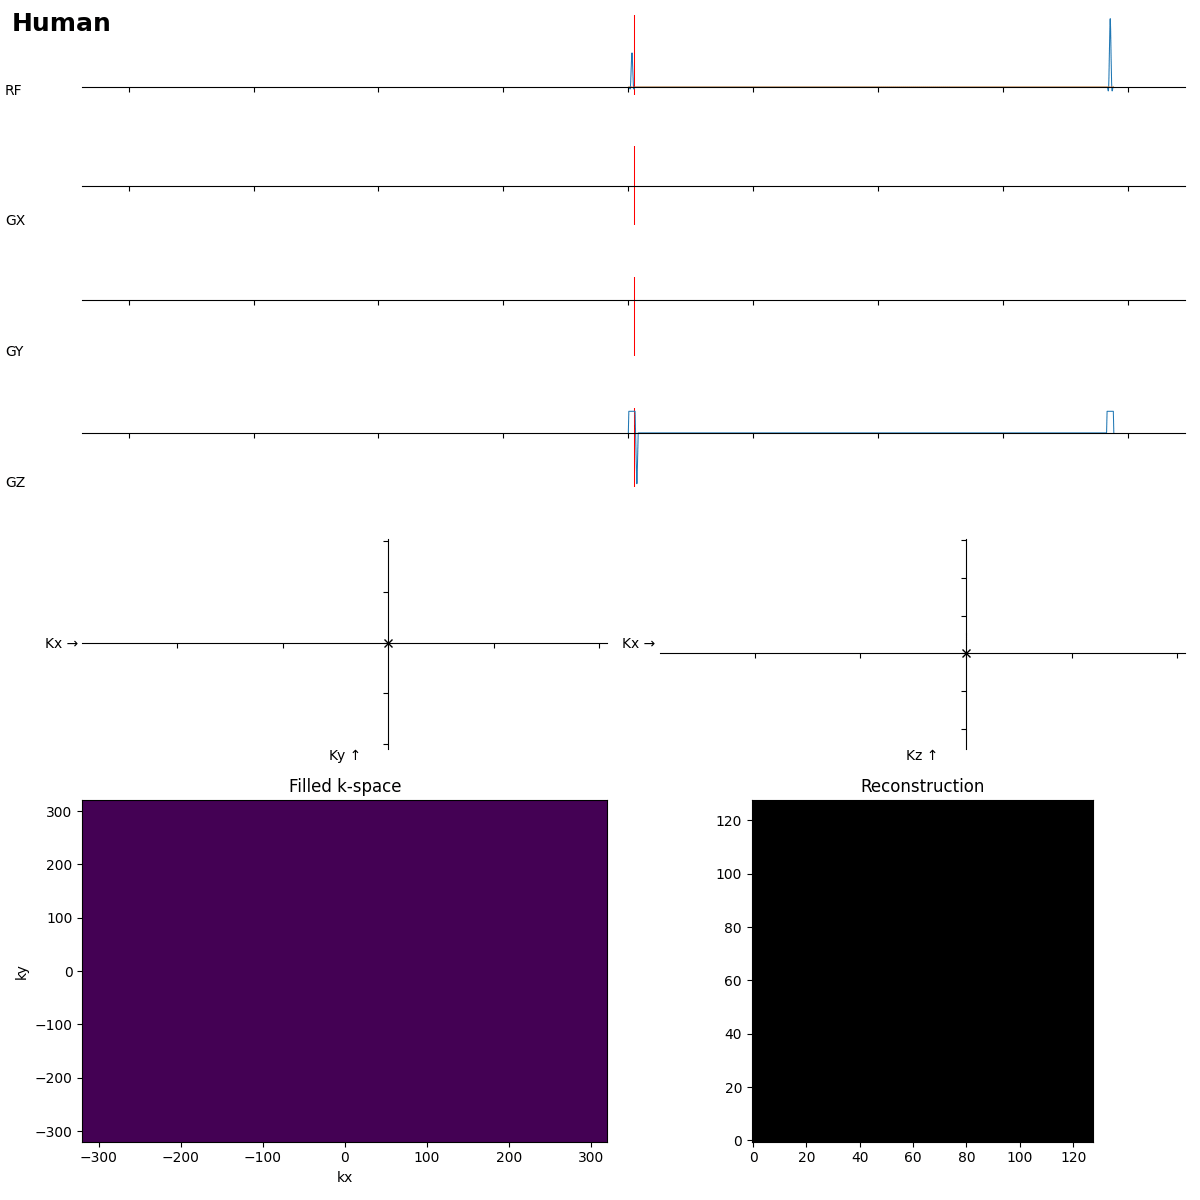
\includegraphics[height=.78\textheight]{img_08_02.png}
\end{center}
\end{frame}

\begin{frame}[t]{Was ist agentische KI?}{Versuch von GPT-4o}
\begin{center}
  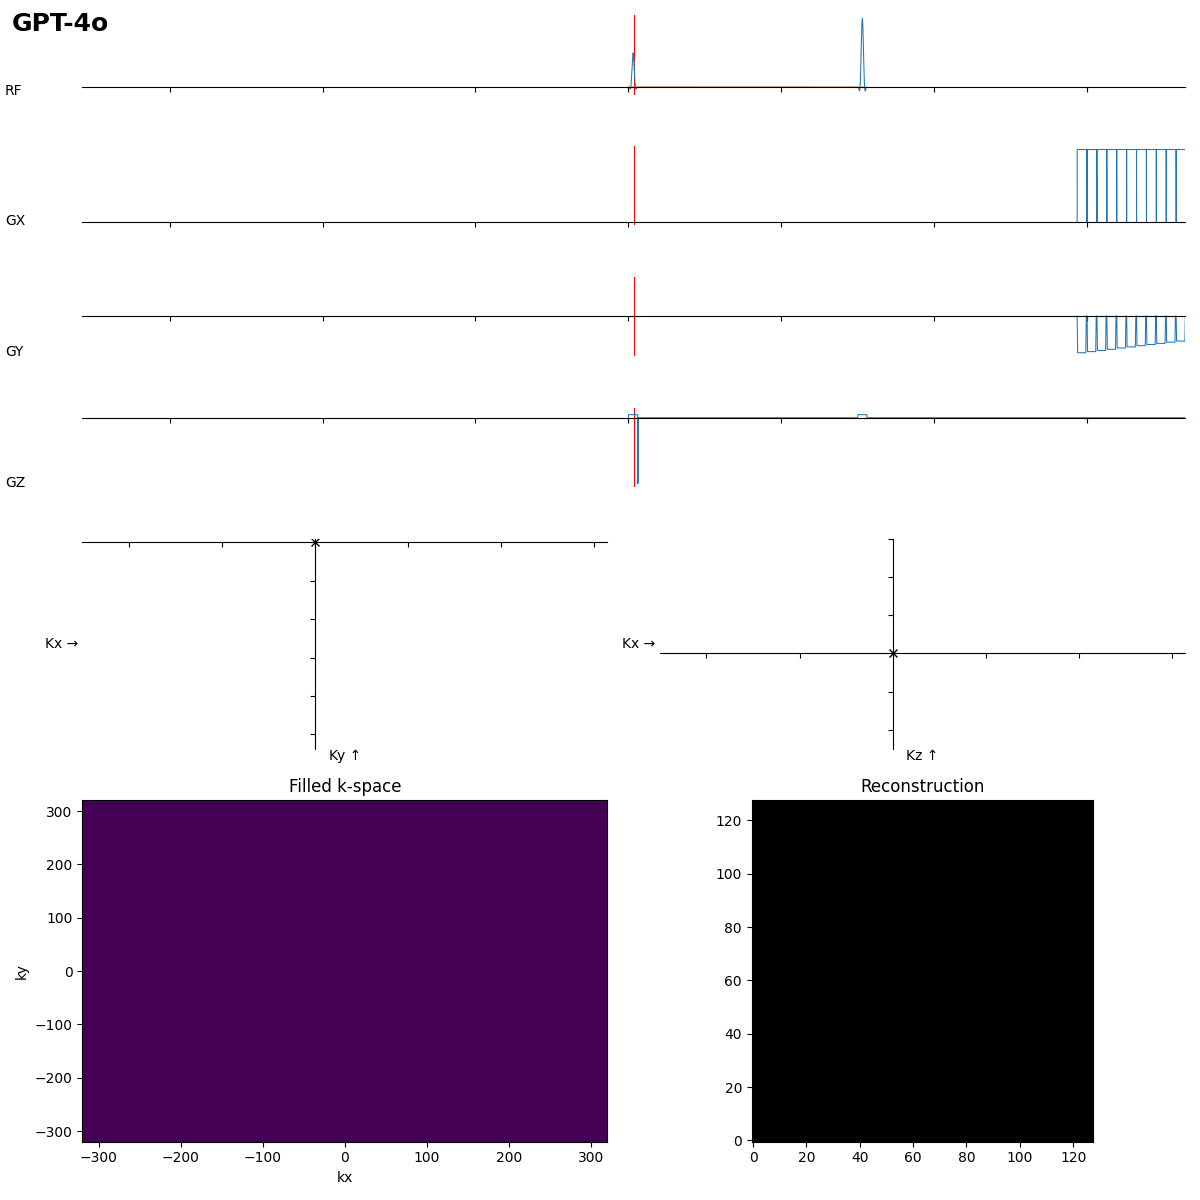
\includegraphics[height=.78\textheight]{img_08_03.png}
\end{center}
\end{frame}

\begin{frame}[t]{Was ist agentische KI?}{Versuch von GROK-3-think}
\begin{center}
  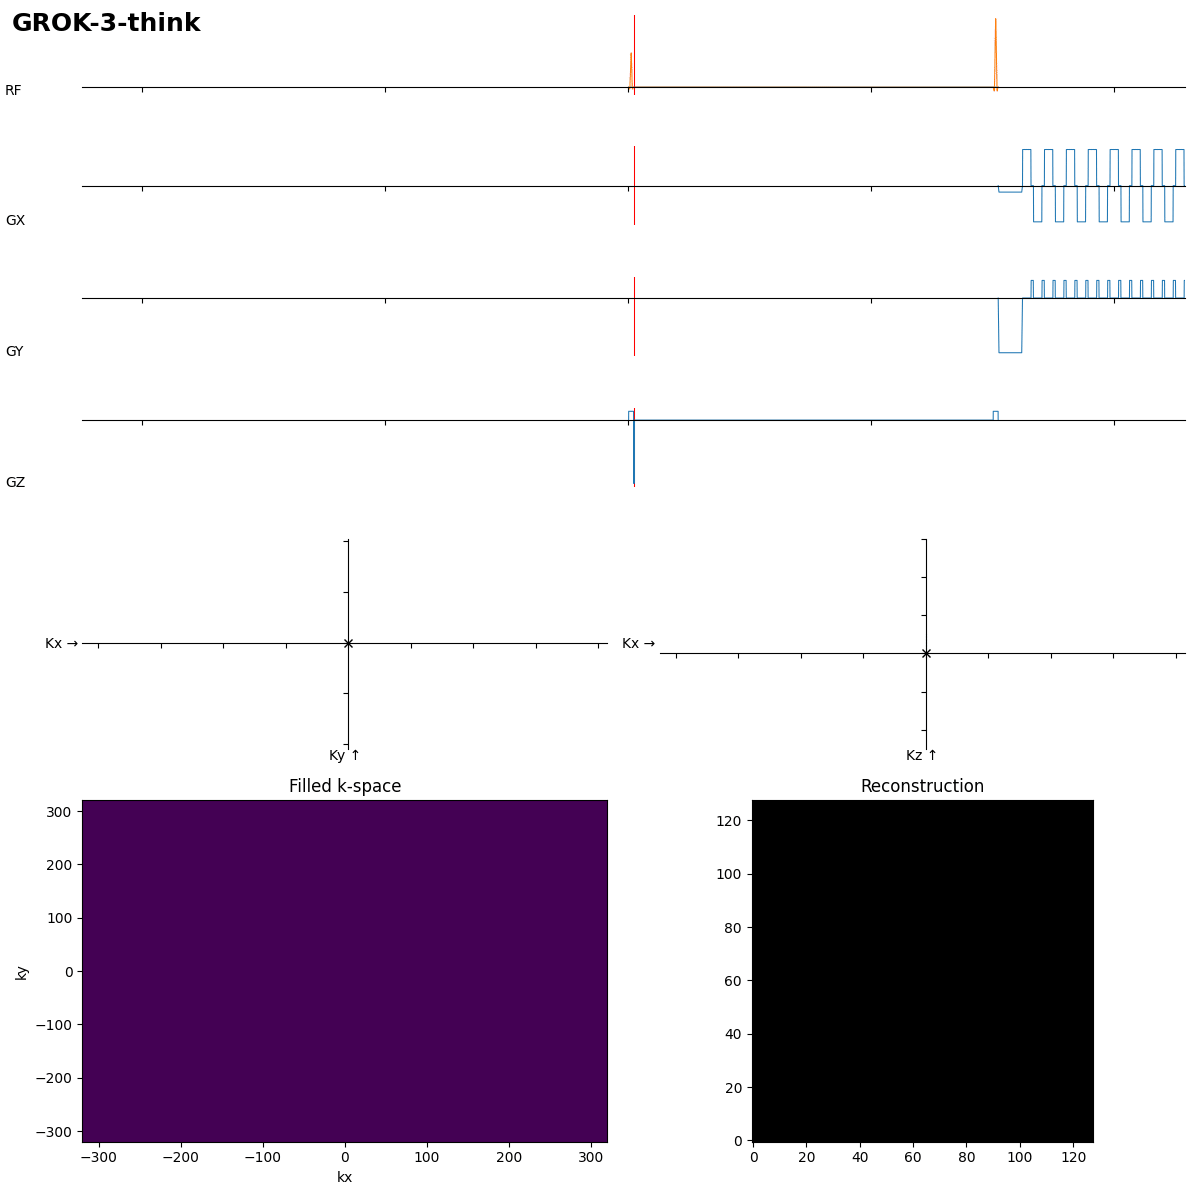
\includegraphics[height=.78\textheight]{img_08_04.png}
\end{center}
\end{frame}

% --------------------------------------------------------------------------
% Abschnittstrenner vor Agent4MR-Ergebnissen
% --------------------------------------------------------------------------
\begin{frame}[t,title]{-}
Wie sieht echte agentische KI aus?
\end{frame}

% --------------------------------------------------------------------------
% Folie 10 - Agent4MR-Ergebnisse (4 Unterfolien)
% --------------------------------------------------------------------------
\begin{frame}[t]{Was ist agentische KI?}{LLM vs.\ Agent4MR}
\begin{center}
  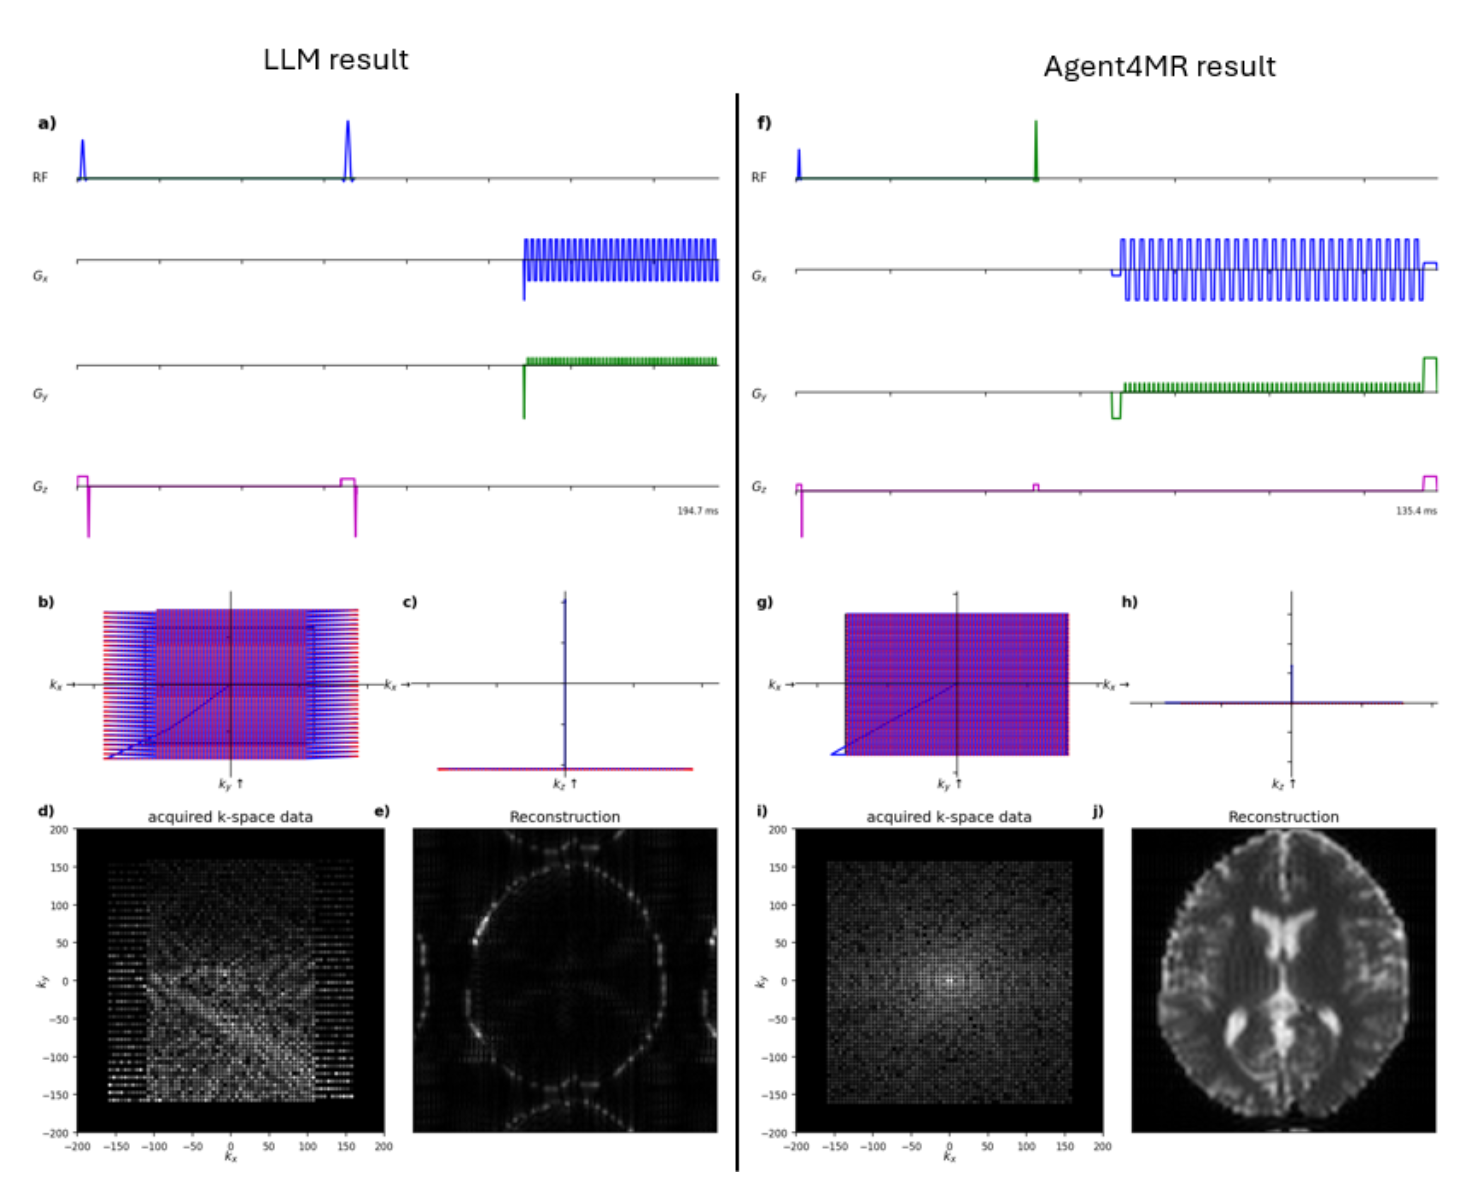
\includegraphics[height=.78\textheight]{img_09_01.png}
\end{center}
\end{frame}

\begin{frame}[t]{Was ist agentische KI?}{Interaktionen pro Modell}
\begin{center}
  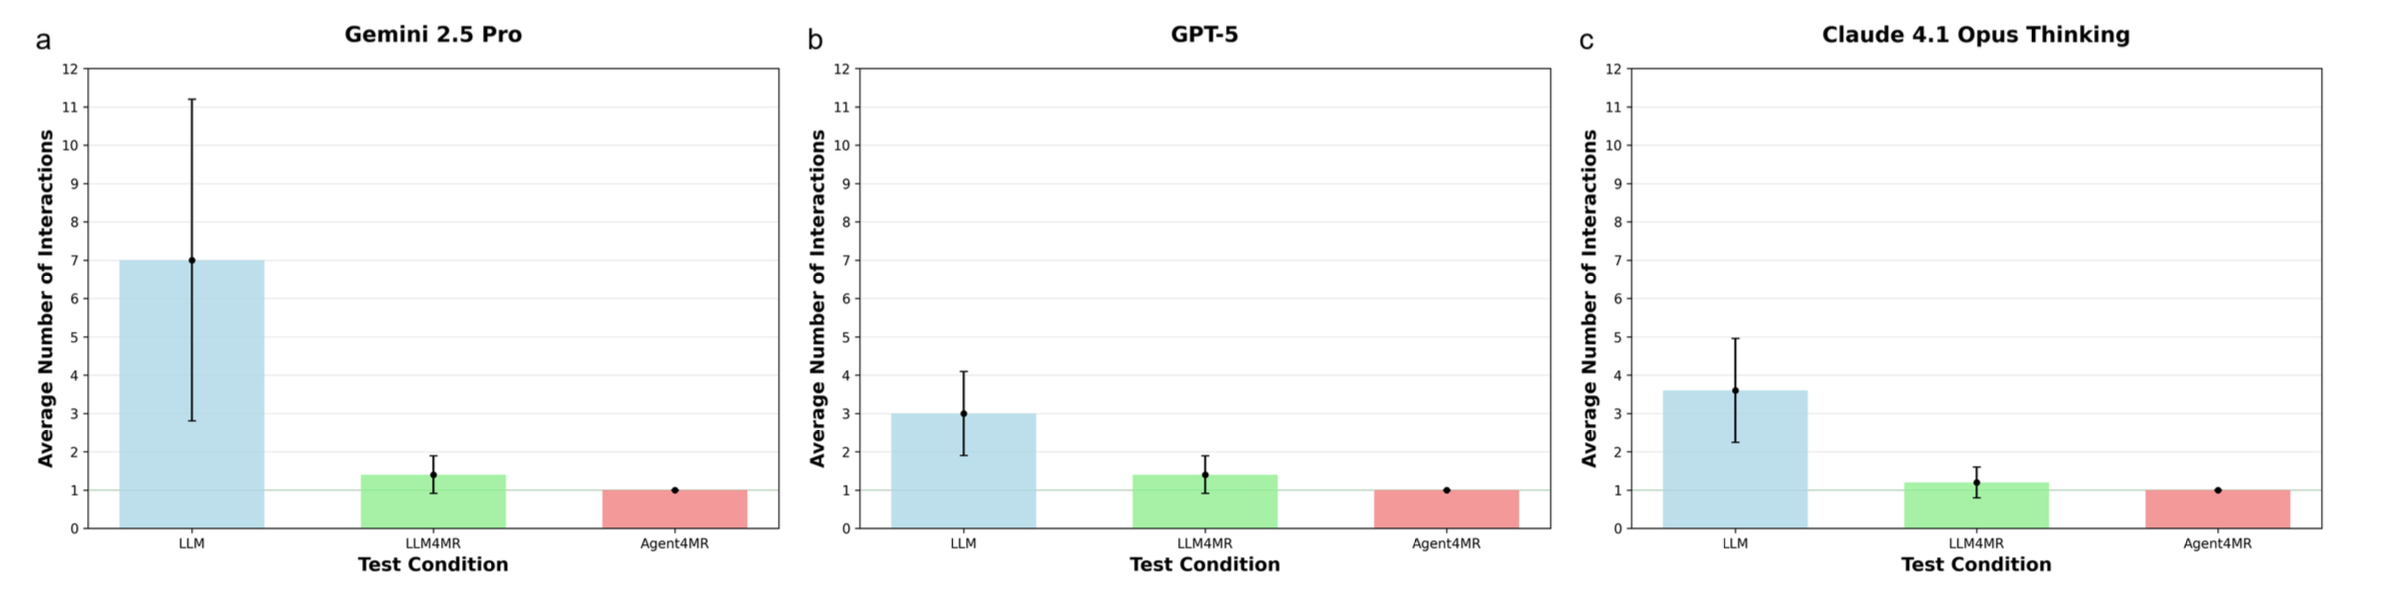
\includegraphics[width=.92\textwidth]{img_09_02.png}
\end{center}
\end{frame}

\begin{frame}[t]{Was ist agentische KI?}{Kostenvergleich}
\begin{center}
  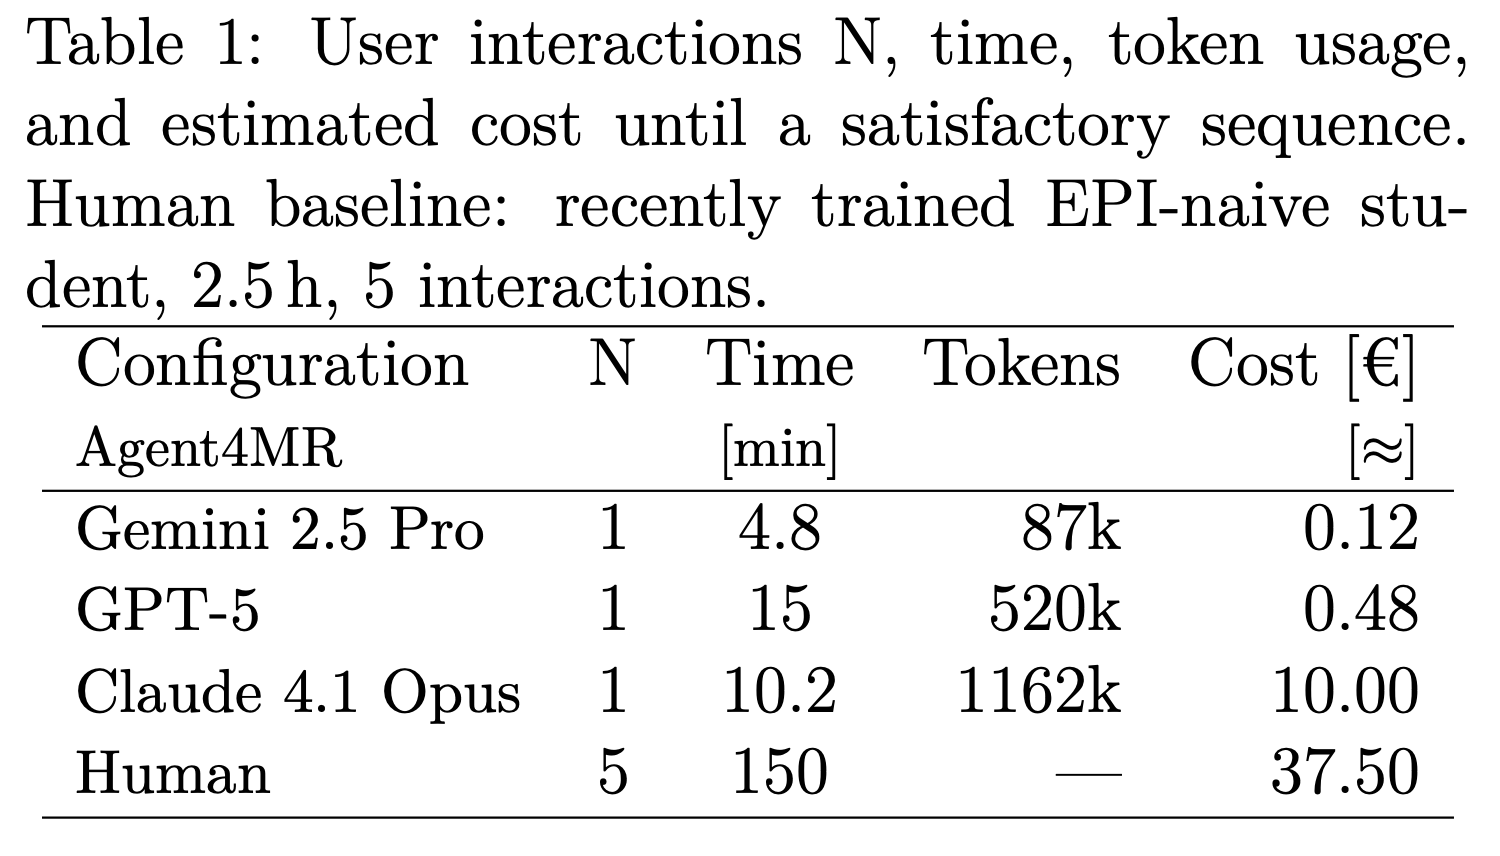
\includegraphics[height=.78\textheight]{img_09_03.png}
\end{center}
\end{frame}

\begin{frame}[t]{Was ist agentische KI?}{Iterativer Fortschritt}
\begin{columns}[c]
  \begin{column}{0.6\textwidth}
    \centering
    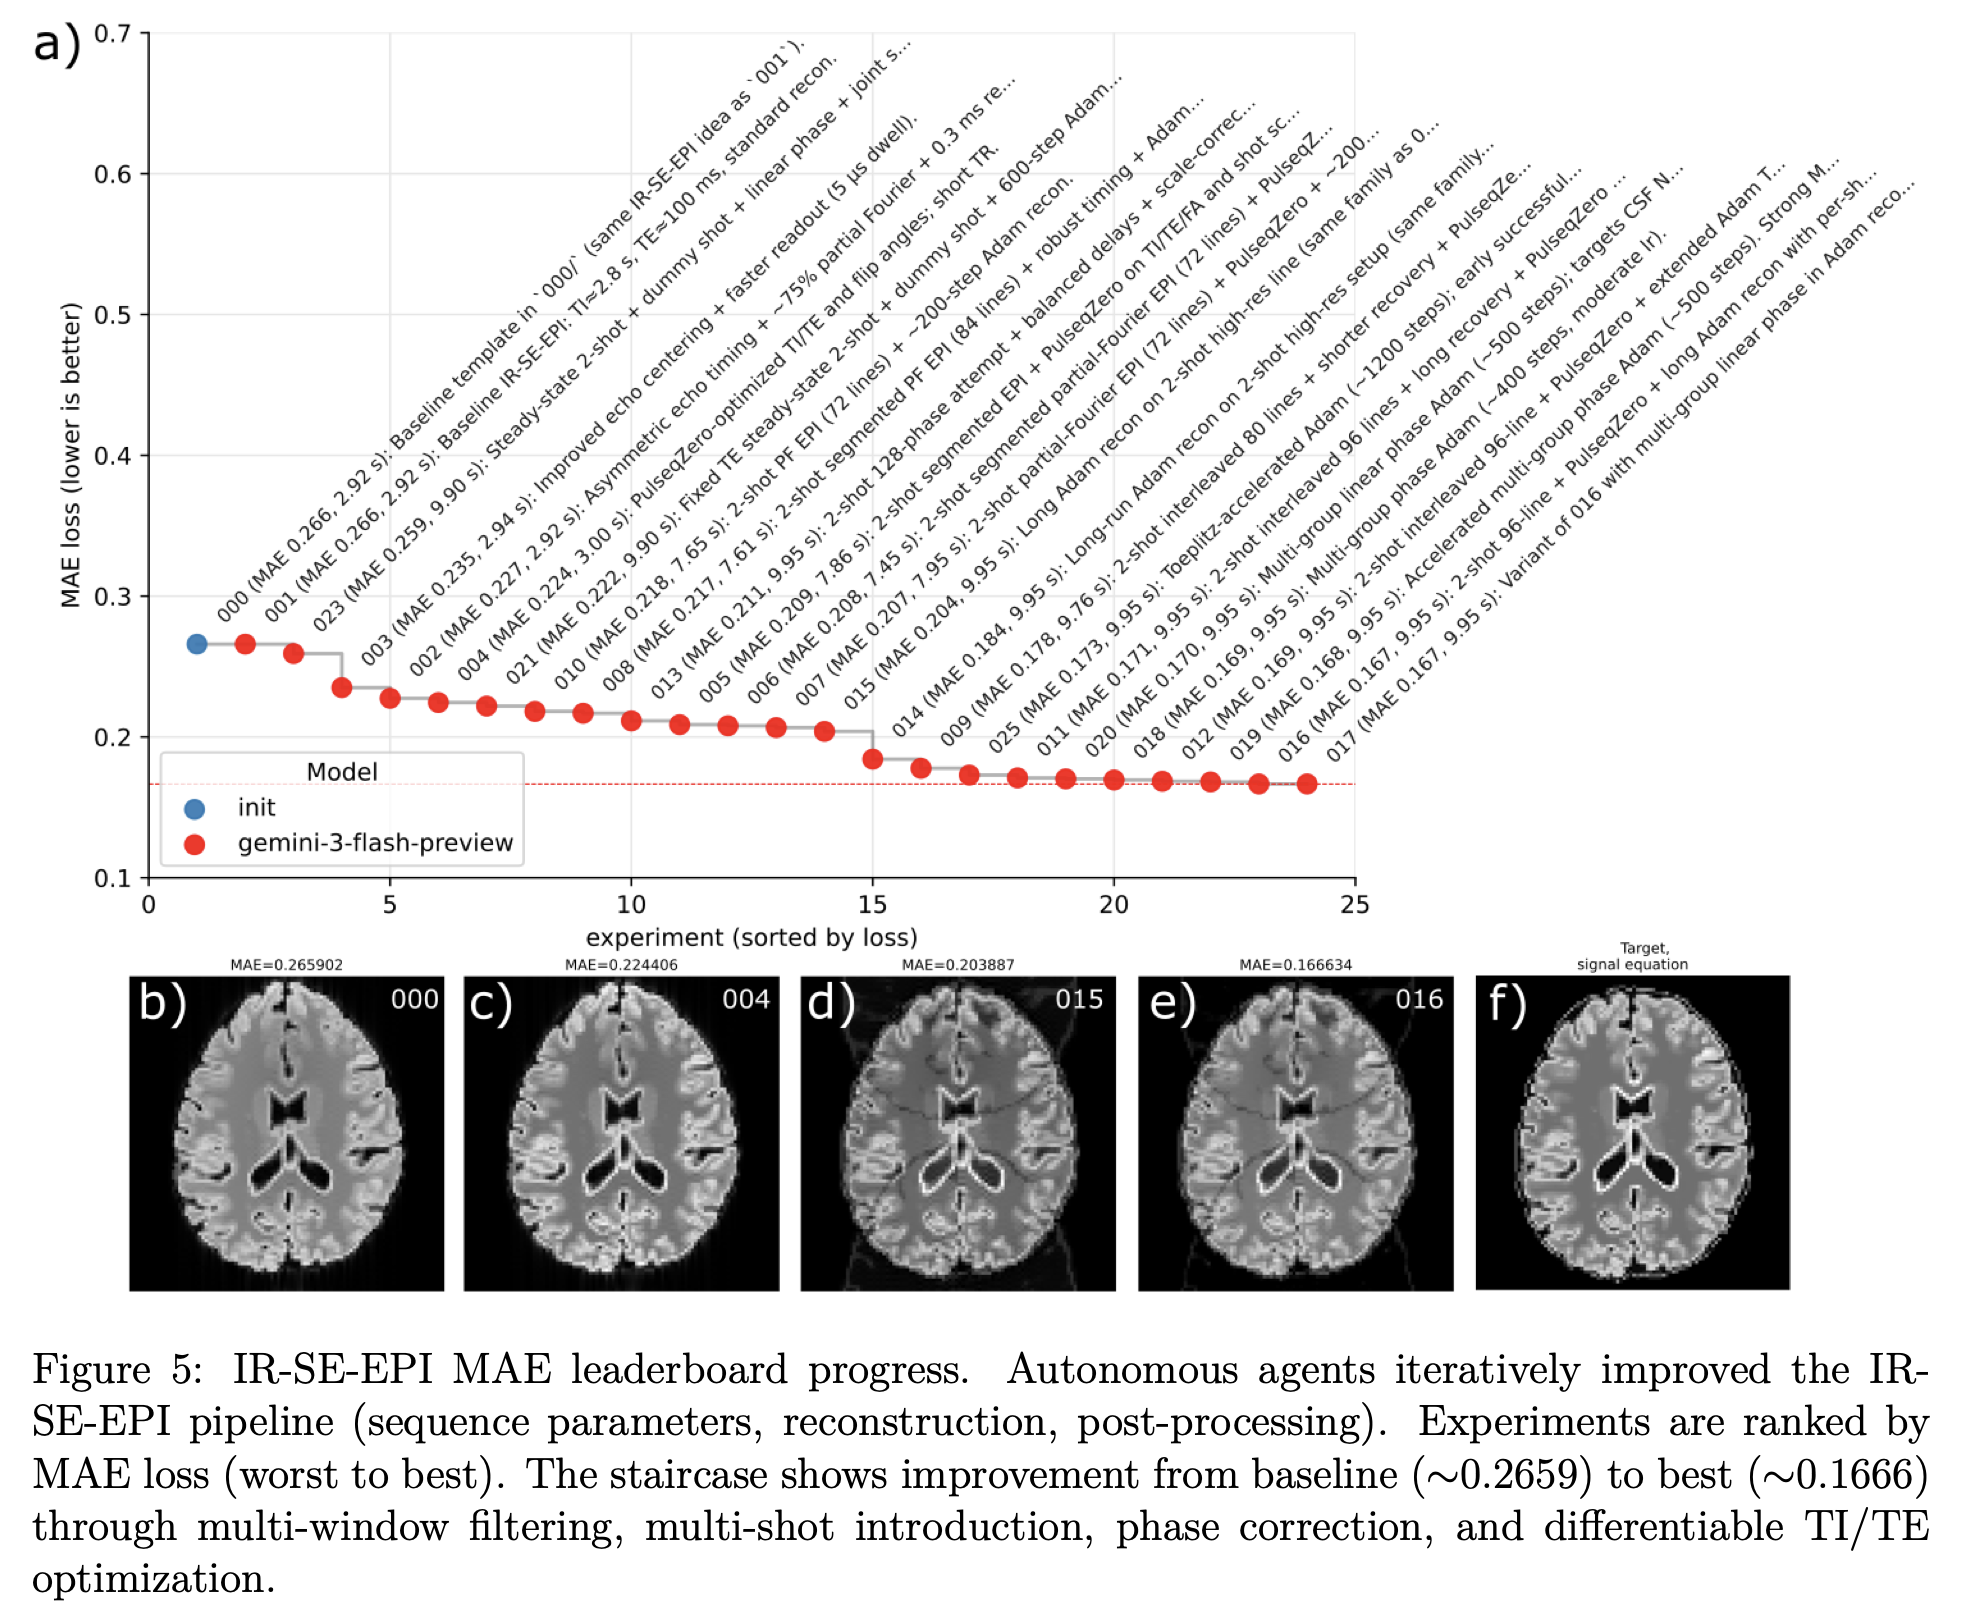
\includegraphics[height=.78\textheight]{img_09_04.png}
  \end{column}
  \begin{column}{0.4\textwidth}
    \centering
    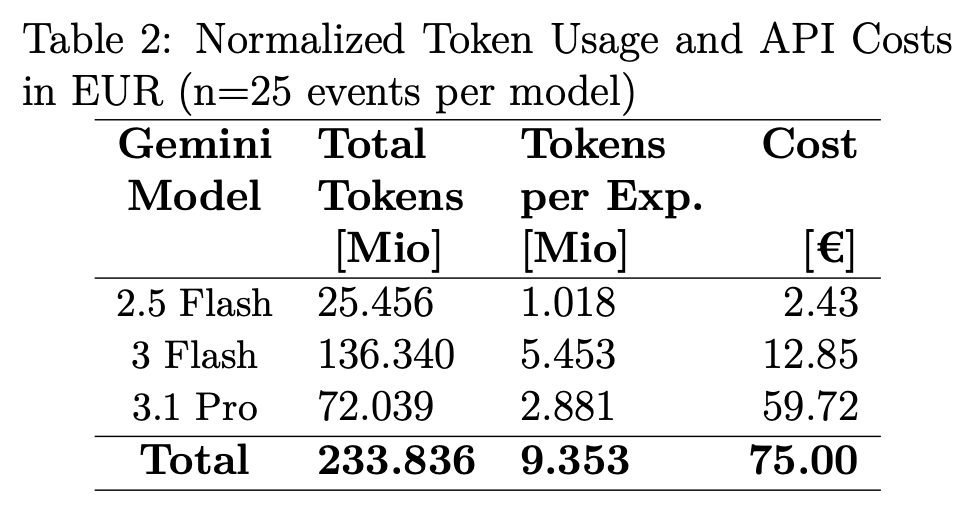
\includegraphics[width=\textwidth]{img_09_05.png}
  \end{column}
\end{columns}
\end{frame}

% --------------------------------------------------------------------------
% Folie 11 - Adaptive KI in der Praxis (3 Unterfolien)
% Reihenfolge: Patienteninformation -> Adaptive Systeme -> Skizze zum Diagramm
% (passt zur überarbeiteten PowerPoint-Variante)
% --------------------------------------------------------------------------
\begin{frame}[t]{Was ist agentische KI?}{Patienteninformation}
\begin{center}
  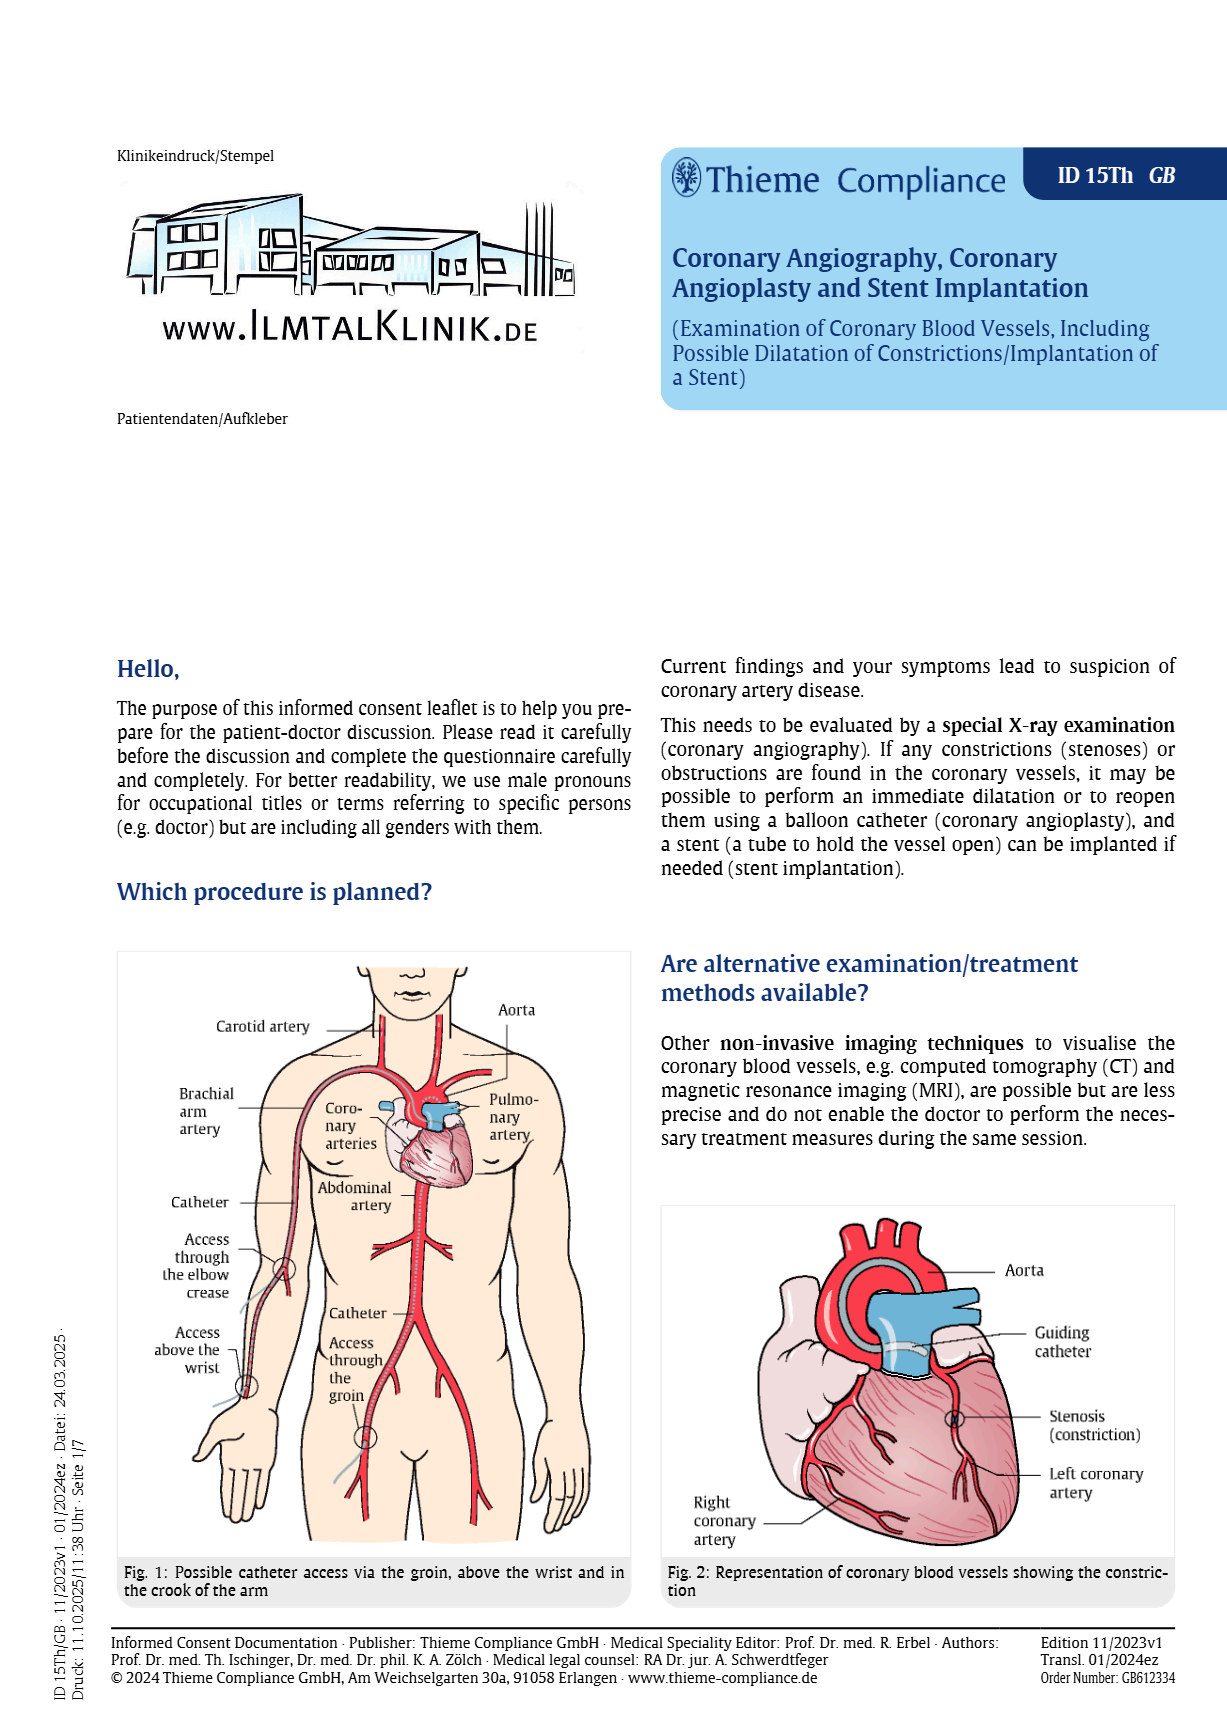
\includegraphics[height=.78\textheight]{img_10_04.png}
\end{center}
\end{frame}

\begin{frame}[t]{Was ist agentische KI?}{Adaptive Systeme}
\begin{center}
  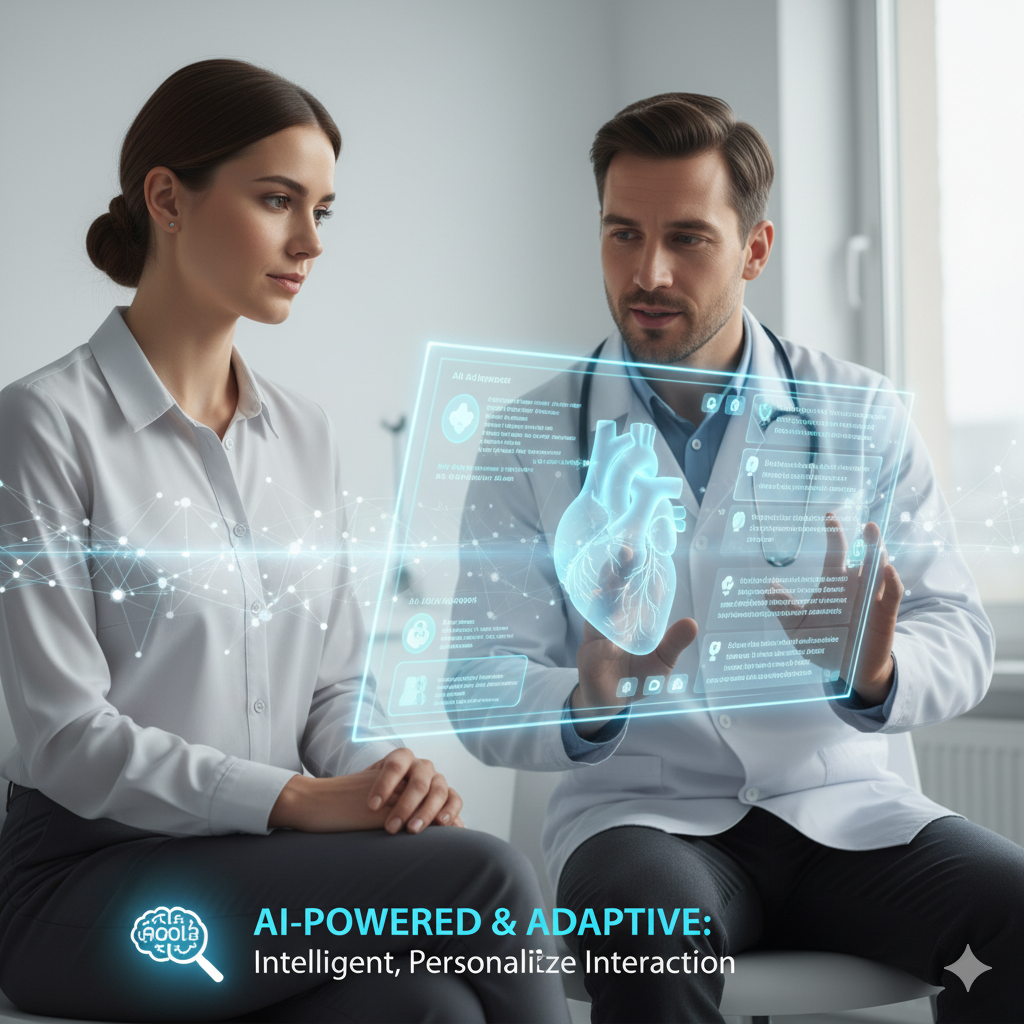
\includegraphics[height=.78\textheight]{img_10_02.png}
\end{center}
\end{frame}

\begin{frame}[t]{Was ist agentische KI?}{Von der Skizze zum Diagramm}
\begin{center}
  \only<1>{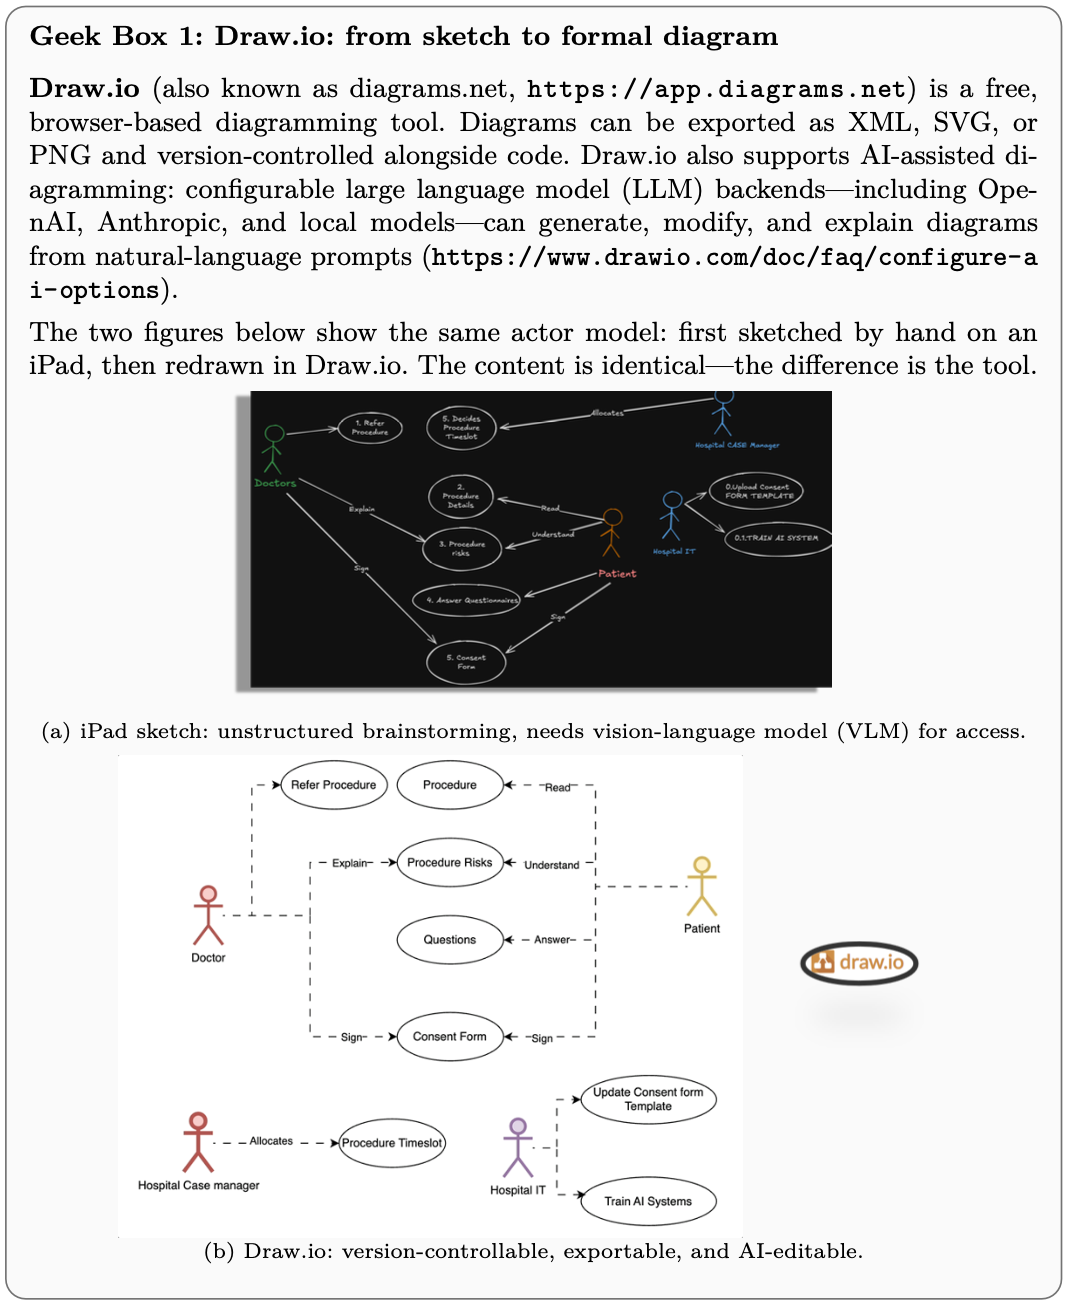
\includegraphics[height=.78\textheight]{img_10_01.png}}%
  \only<2>{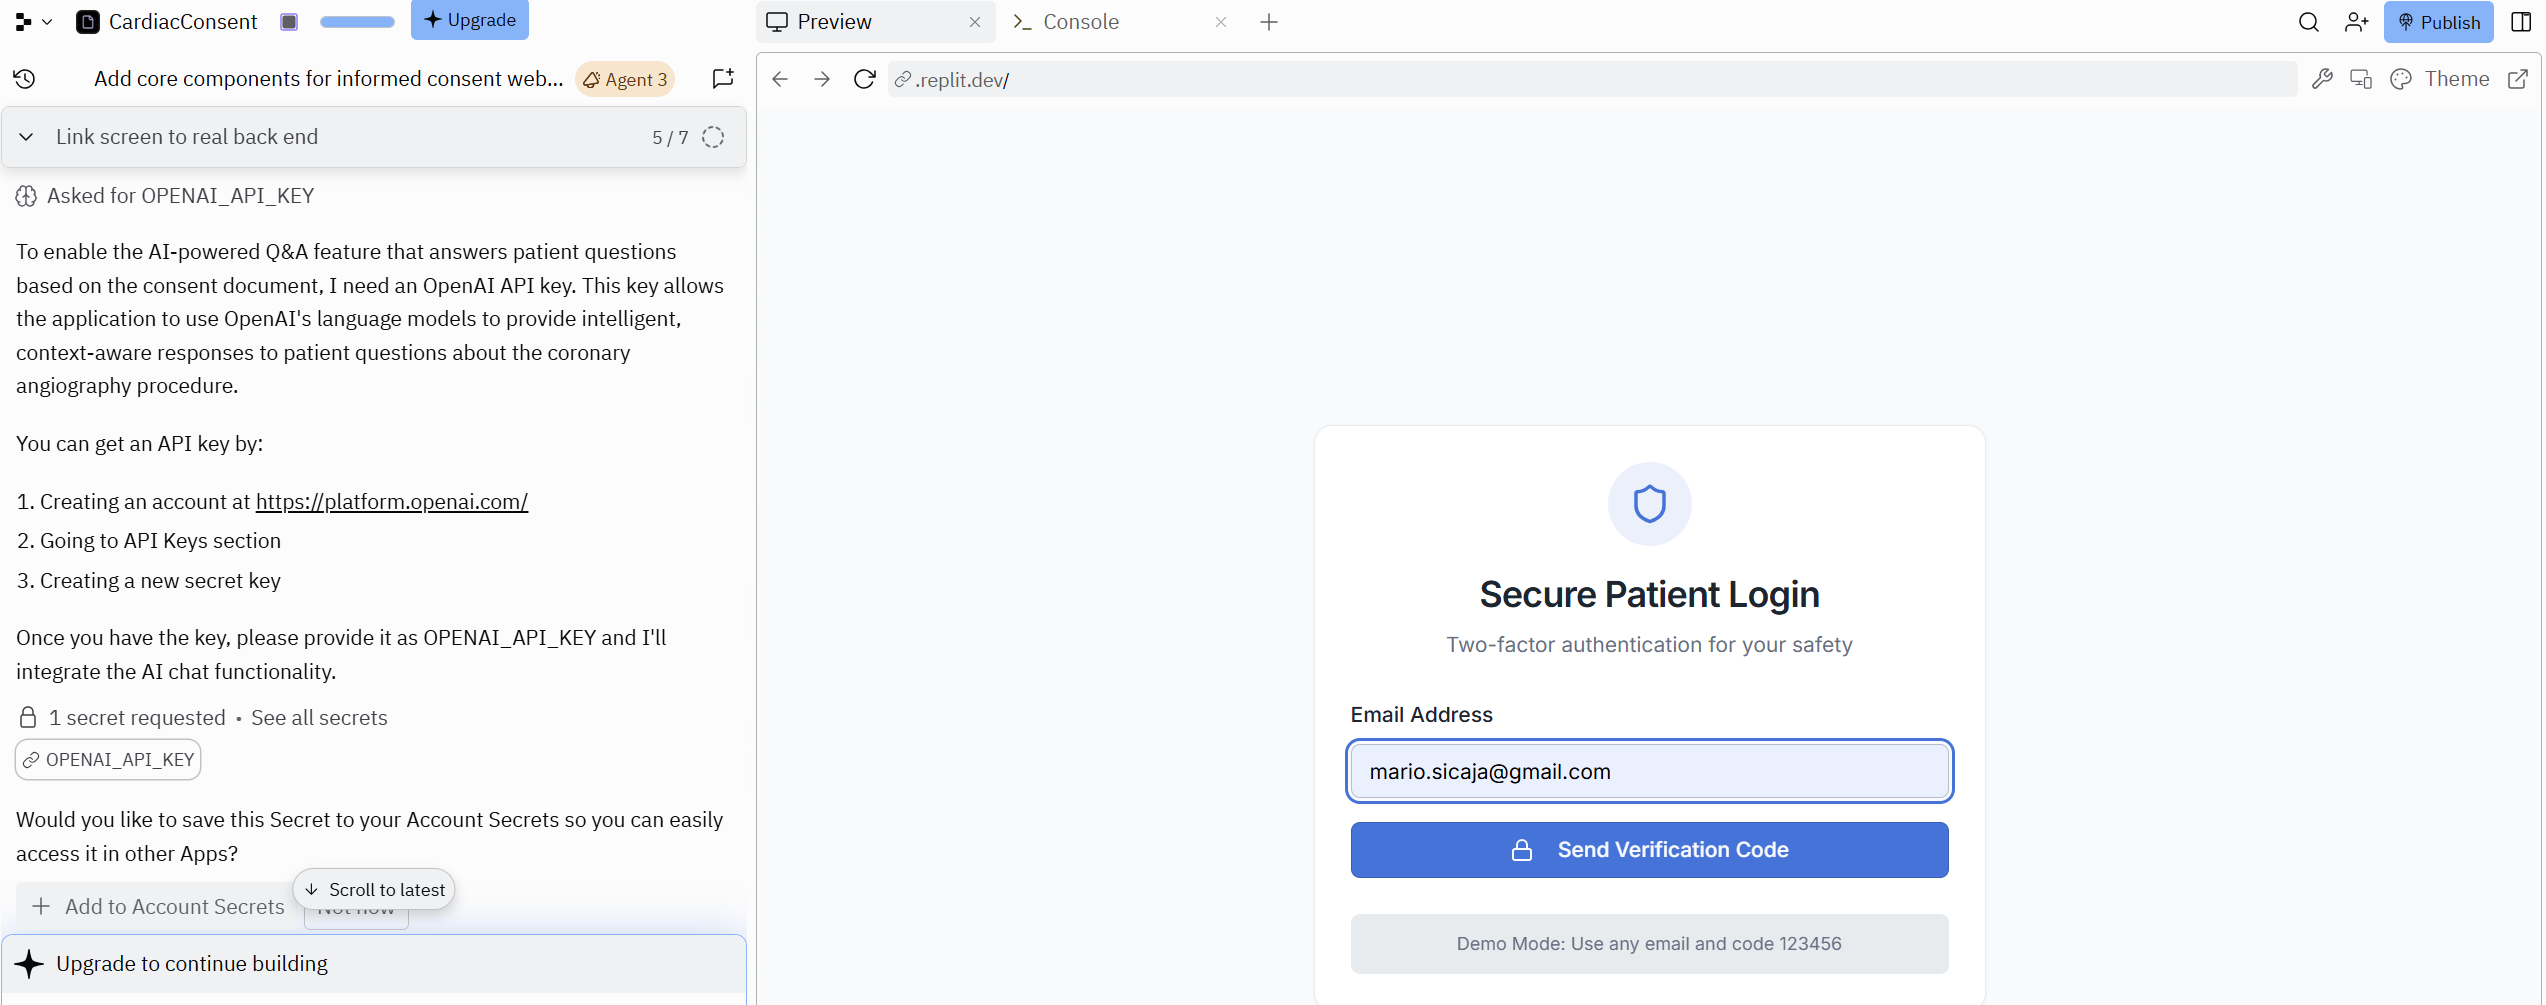
\includegraphics[width=.95\textwidth,keepaspectratio]{img_10_03.png}}
\end{center}
\end{frame}

% --------------------------------------------------------------------------
% Folie 12 - Vibe Coding und fortgeschrittene KI-Techniken (4 Unterfolien)
% --------------------------------------------------------------------------
\begin{frame}[t]{Was ist agentische KI?}{Vibe Coding}
\begin{center}
  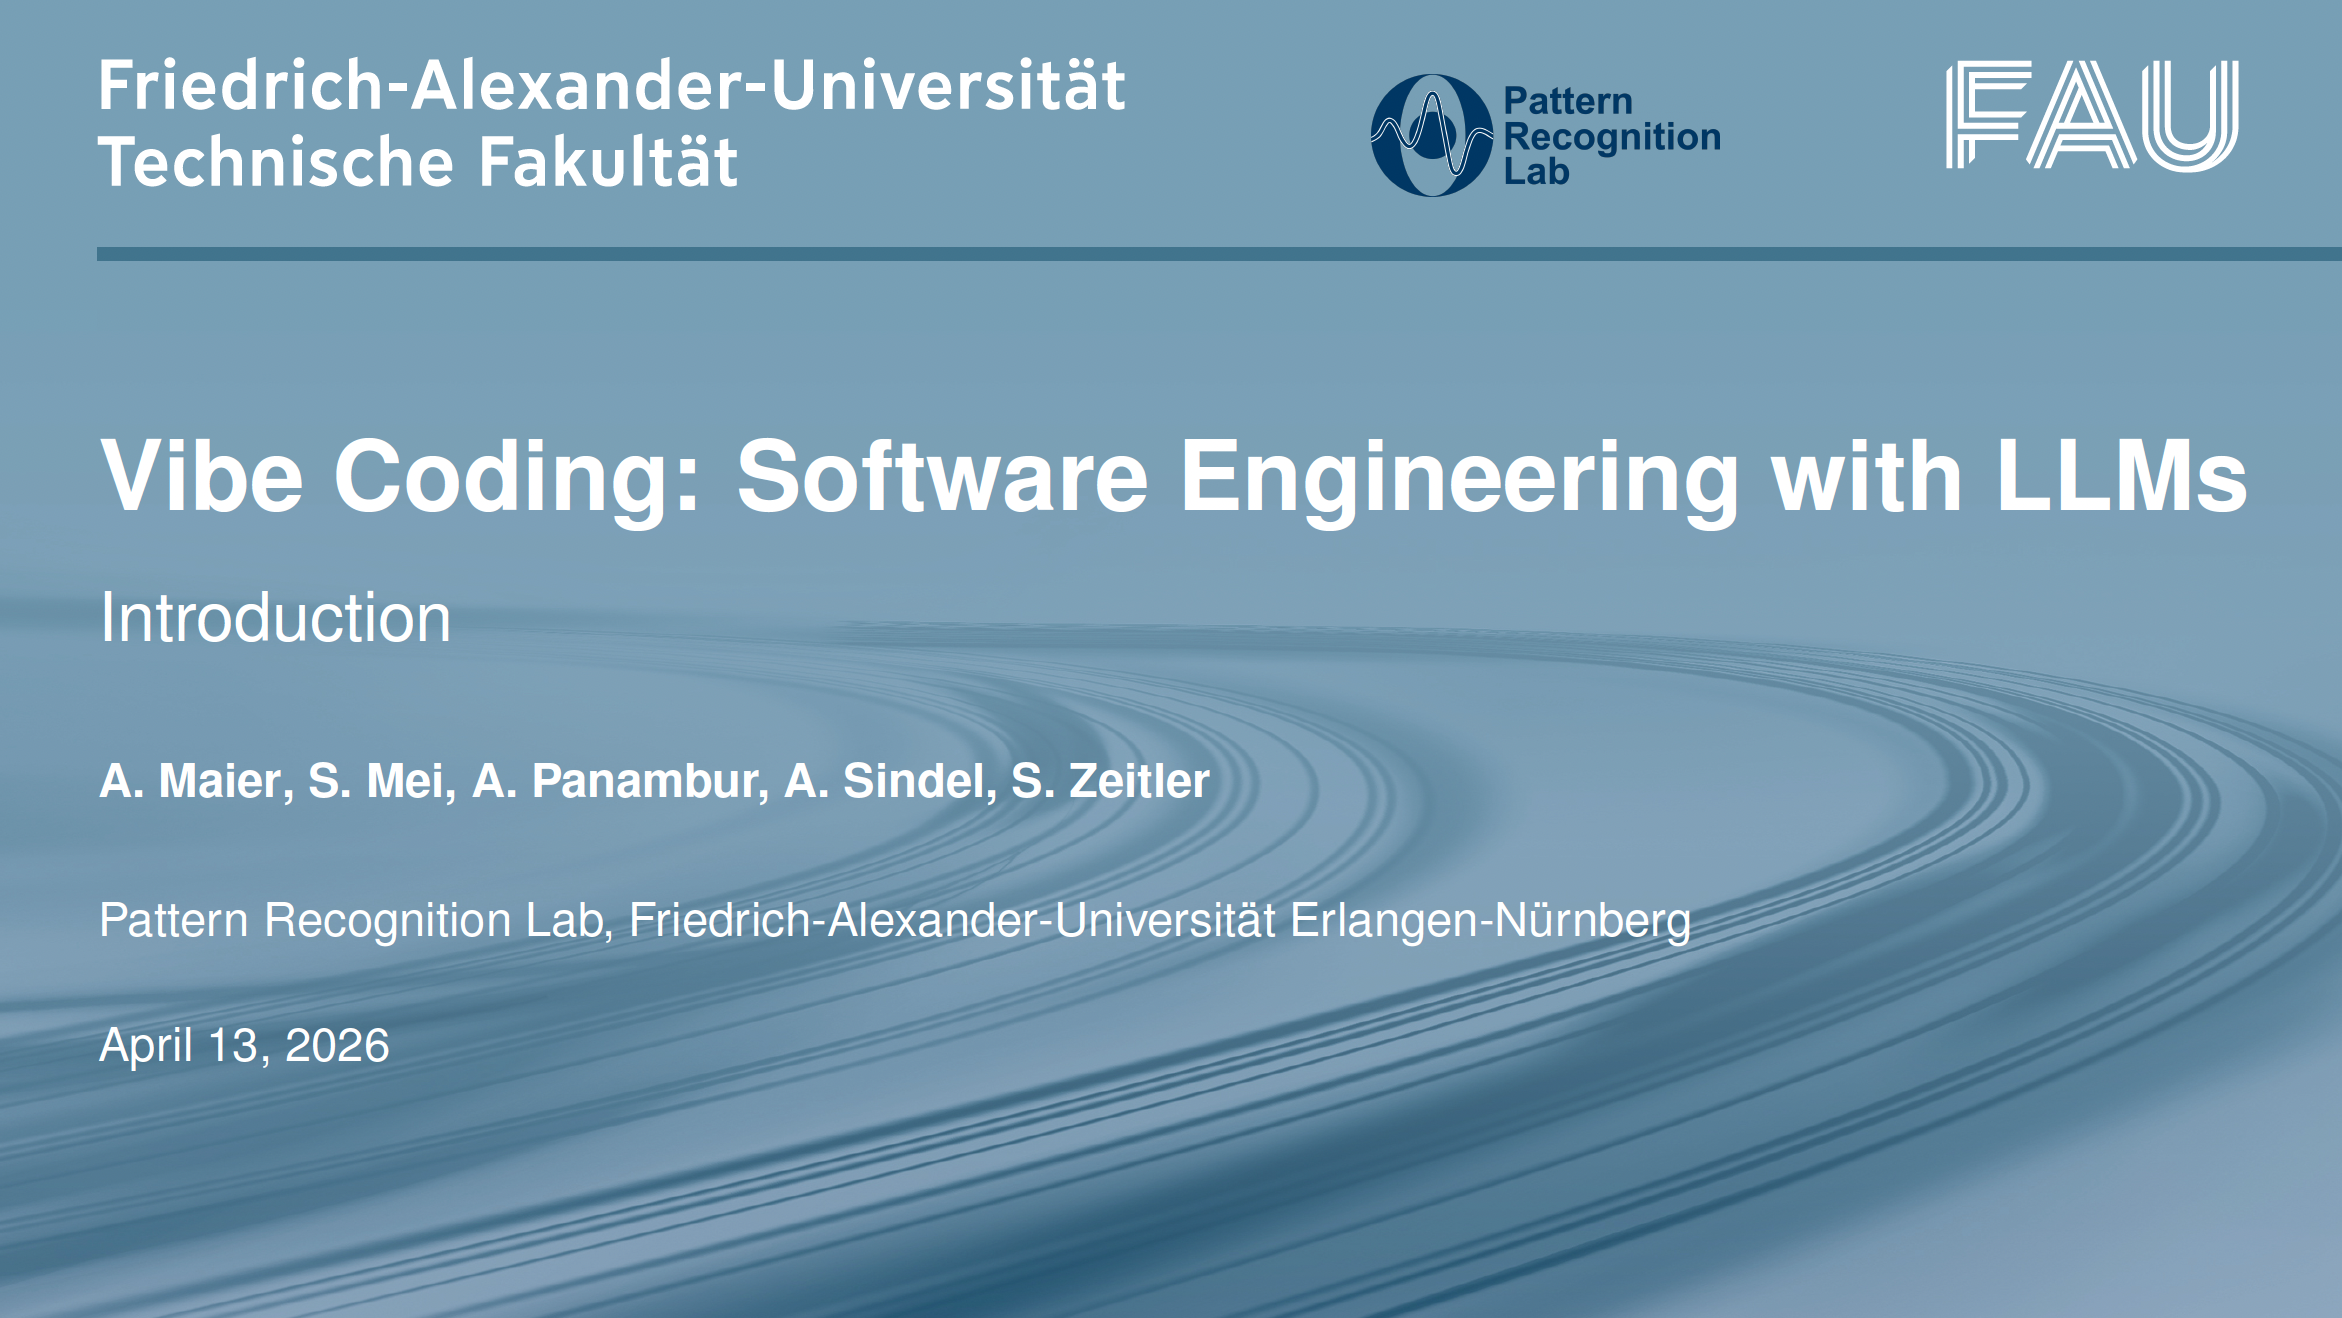
\includegraphics[height=.78\textheight]{img_11_01.png}
\end{center}
\end{frame}

\begin{frame}[t]{Was ist agentische KI?}{Fortgeschrittene KI-gestützte Techniken}
\begin{center}
  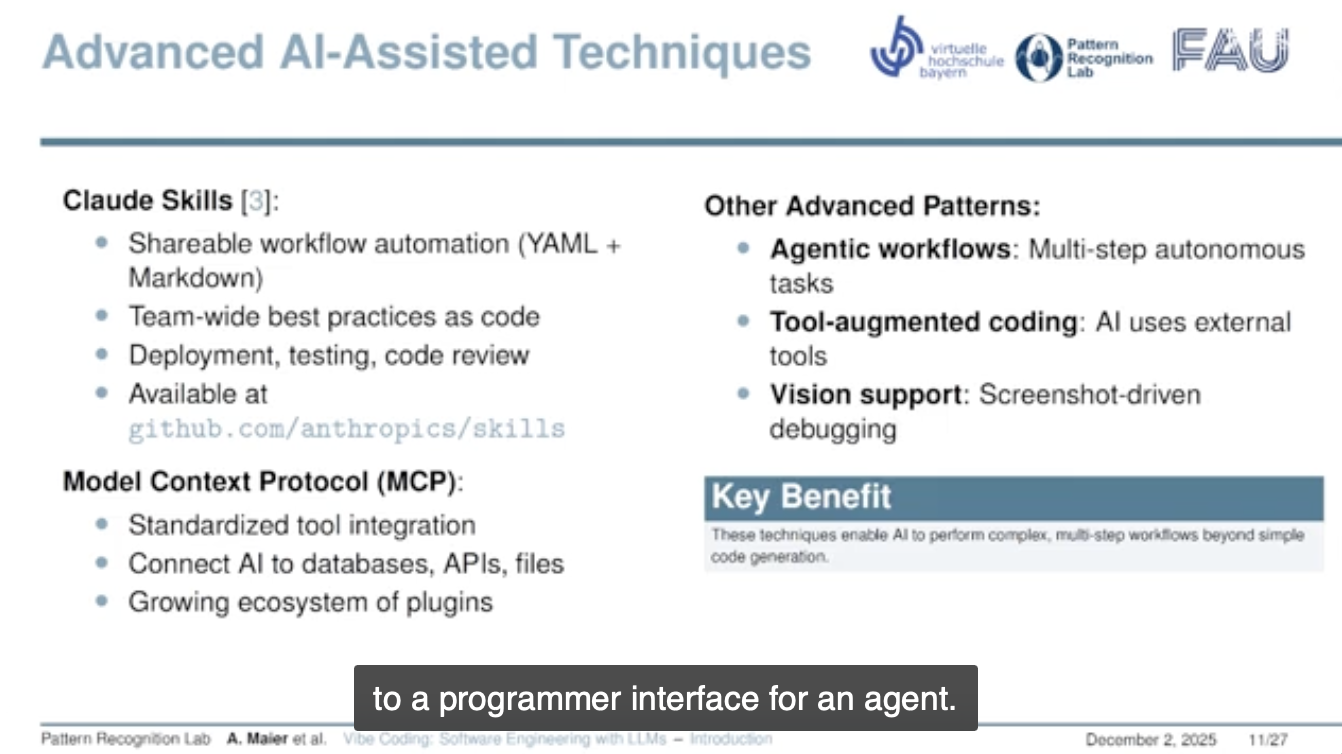
\includegraphics[height=.78\textheight]{img_11_02.png}
\end{center}
\end{frame}

\begin{frame}[t]{Was ist agentische KI?}{Markdown-gesteuerte Qualitätssicherung}
\begin{center}
  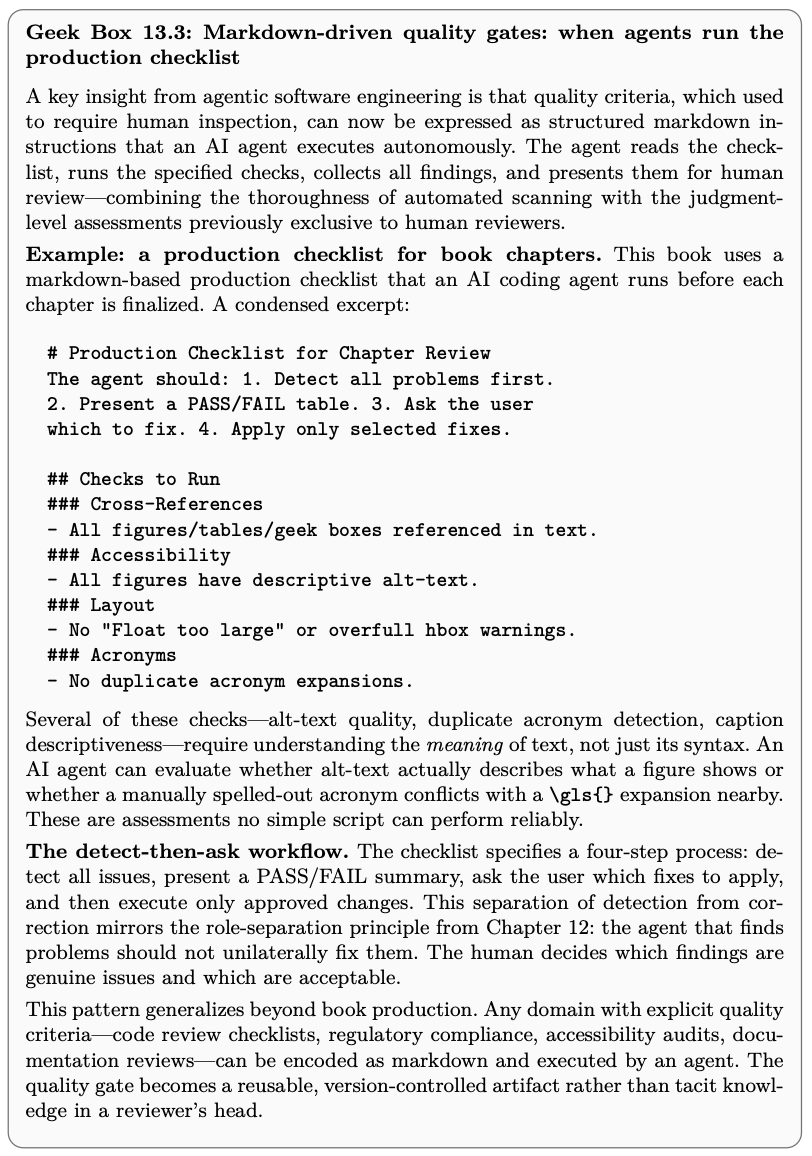
\includegraphics[height=.78\textheight]{img_11_03.png}
\end{center}
\end{frame}

\begin{frame}[t]{Was ist agentische KI?}{Lehrbuch}
\begin{columns}[c]
  \begin{column}{0.5\textwidth}
    \centering
    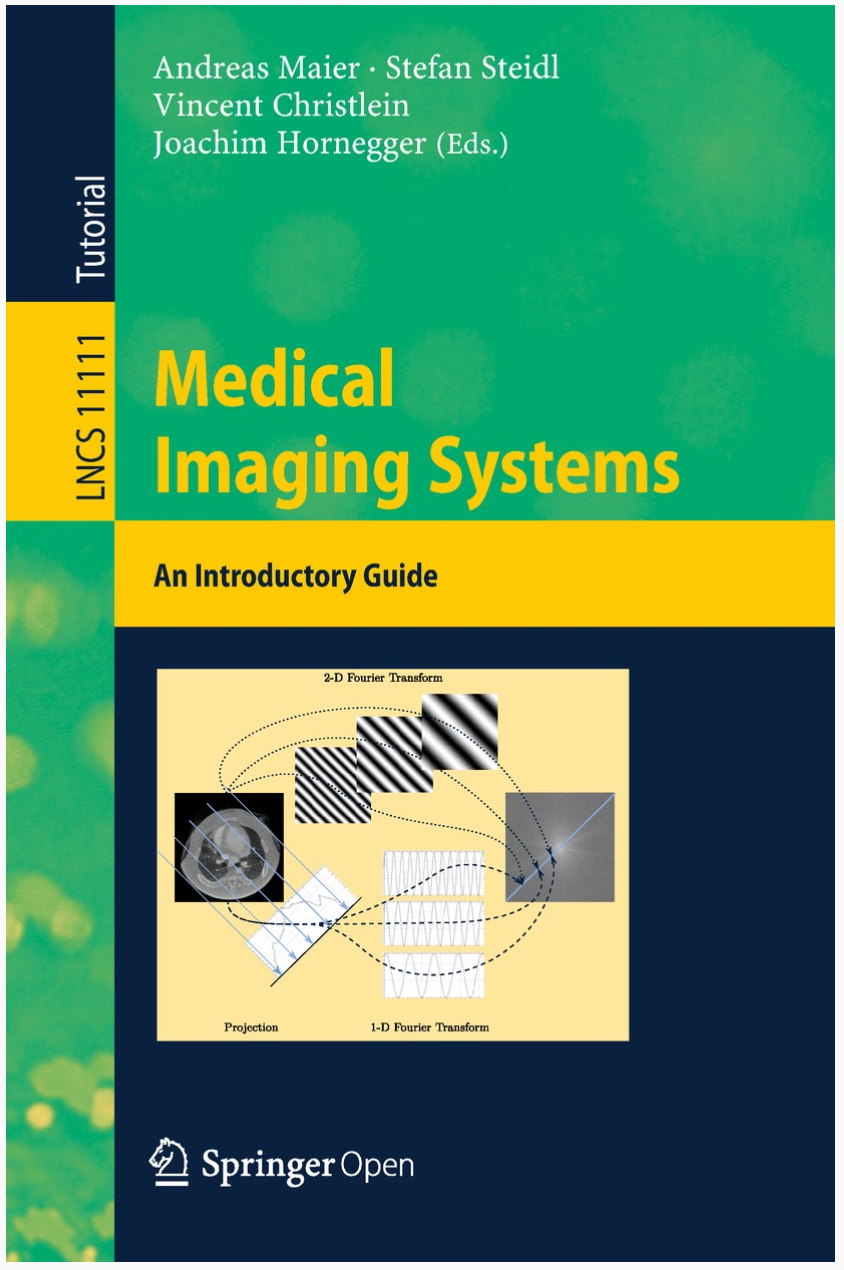
\includegraphics[height=.78\textheight]{img_11_04.png}
  \end{column}
  \begin{column}{0.5\textwidth}
    \centering
    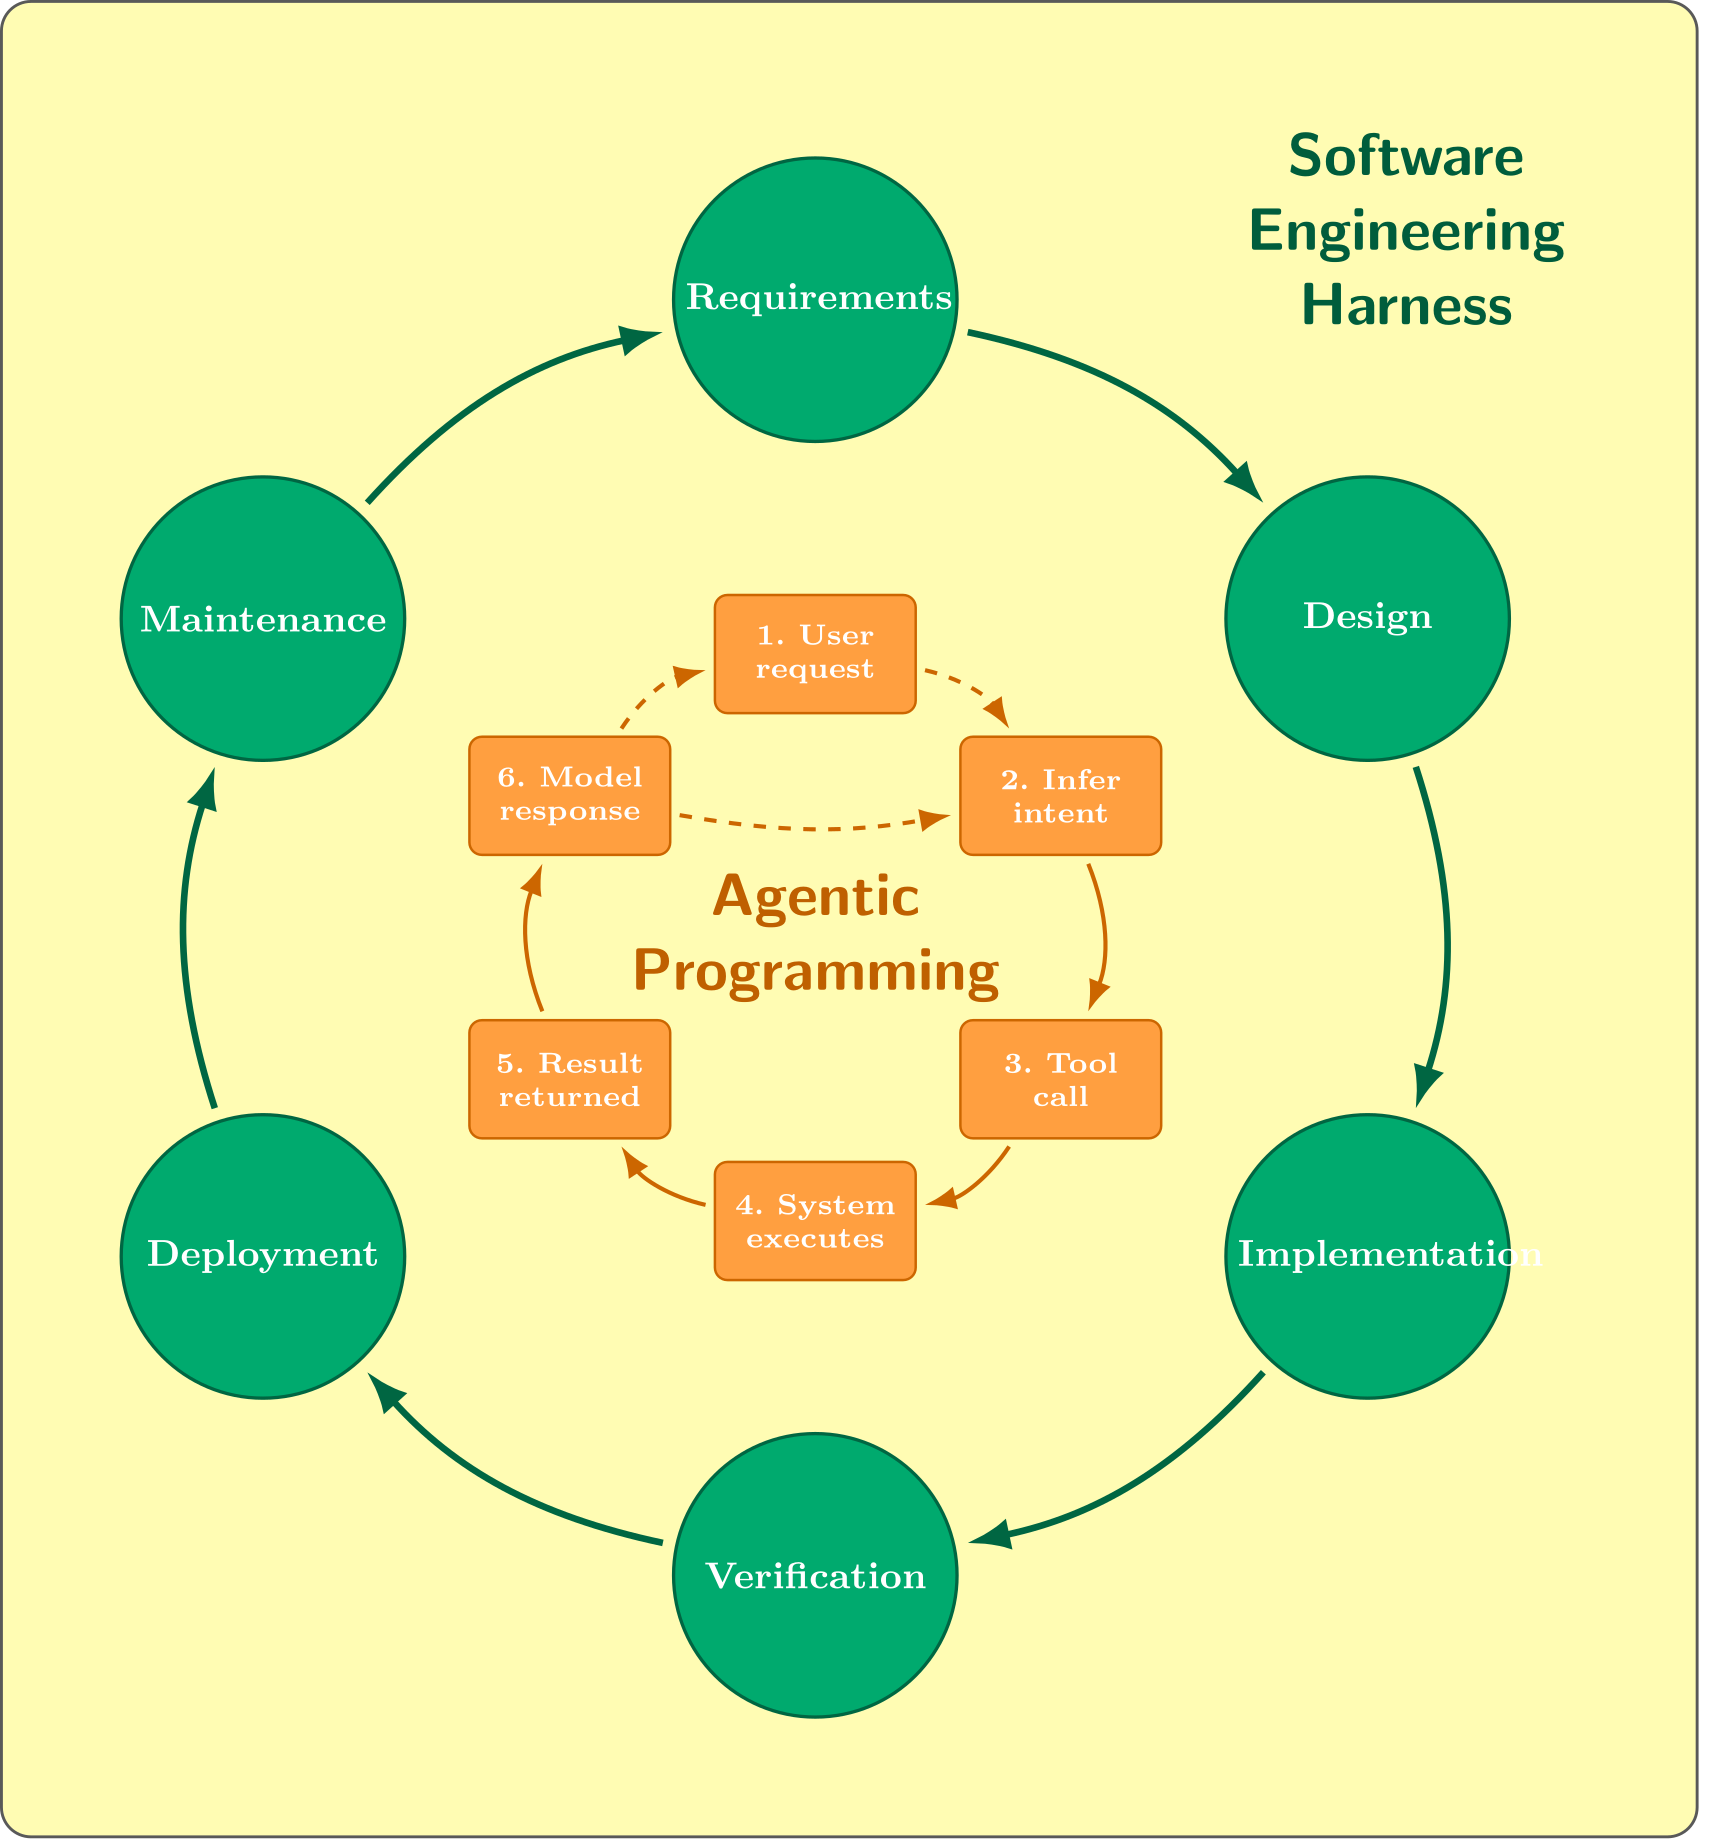
\includegraphics[height=.6\textheight]{img_11_05.png}
  \end{column}
\end{columns}
\end{frame}

% --------------------------------------------------------------------------
% Folie 13 - Abschnittstrenner
% --------------------------------------------------------------------------
\begin{frame}[t,title]{-}
Wie geht es weiter?
\end{frame}

% --------------------------------------------------------------------------
% Folie 14 - Fast alles ist jetzt einfach (4 Unterfolien)
% --------------------------------------------------------------------------
\begin{frame}[t]{Fast alles ist jetzt einfach\dots}{China und KI}
\begin{center}
  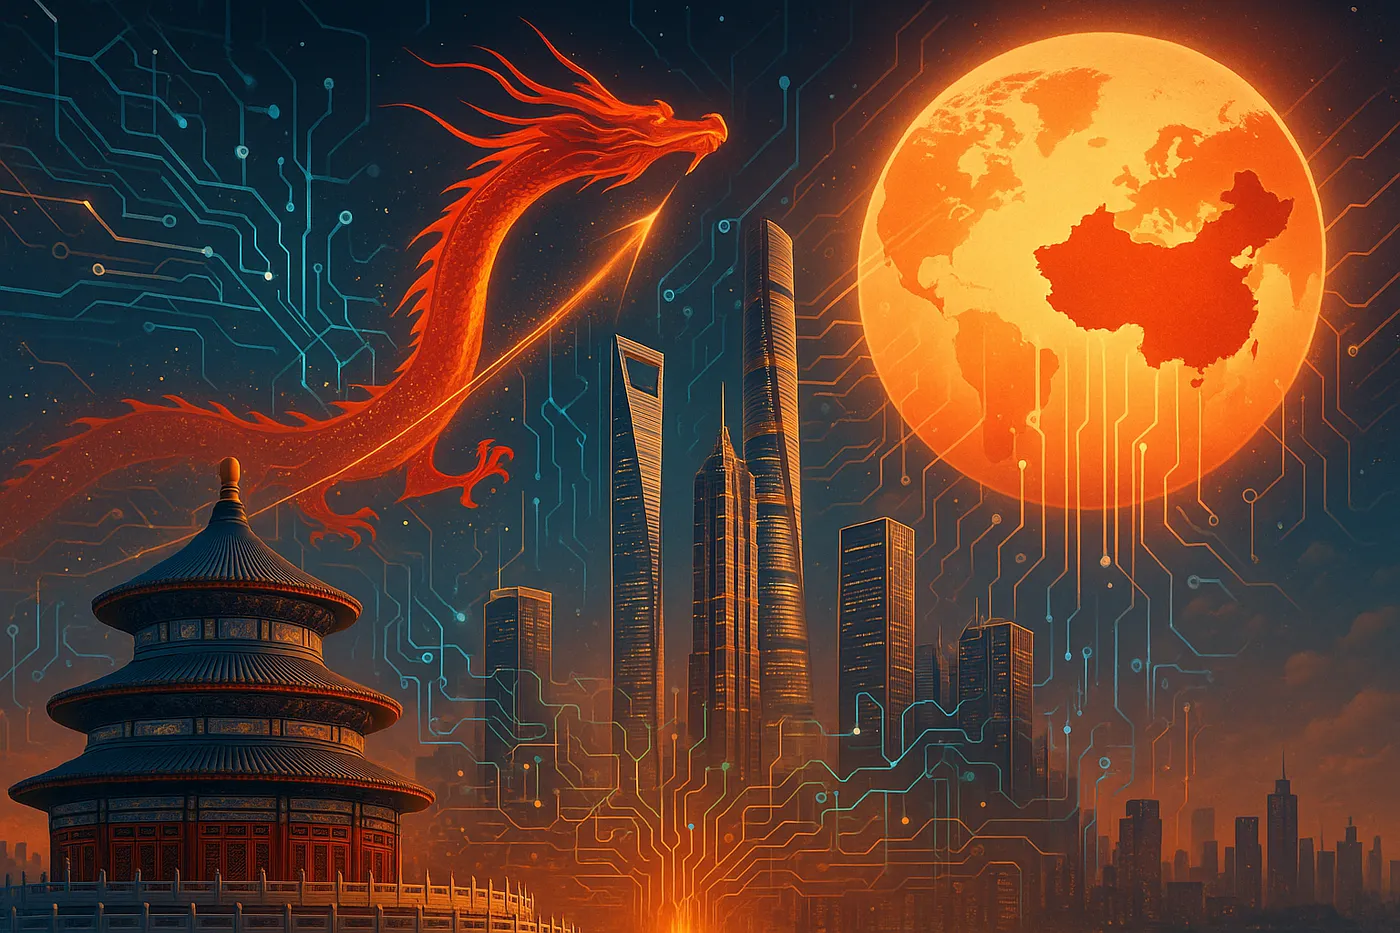
\includegraphics[height=.78\textheight]{img_13_01.png}
\end{center}
\end{frame}

\begin{frame}[t]{Fast alles ist jetzt einfach\dots}{Konferenzanteile}
\begin{center}
  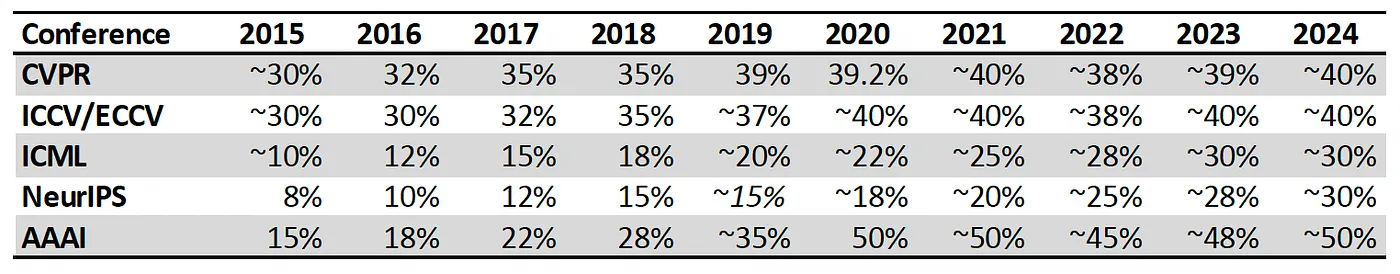
\includegraphics[width=.9\textwidth]{img_13_02.png}
\end{center}
\end{frame}

\begin{frame}[t]{Fast alles ist jetzt einfach\dots}{ConferenceStats-Workflow}
\begin{center}
  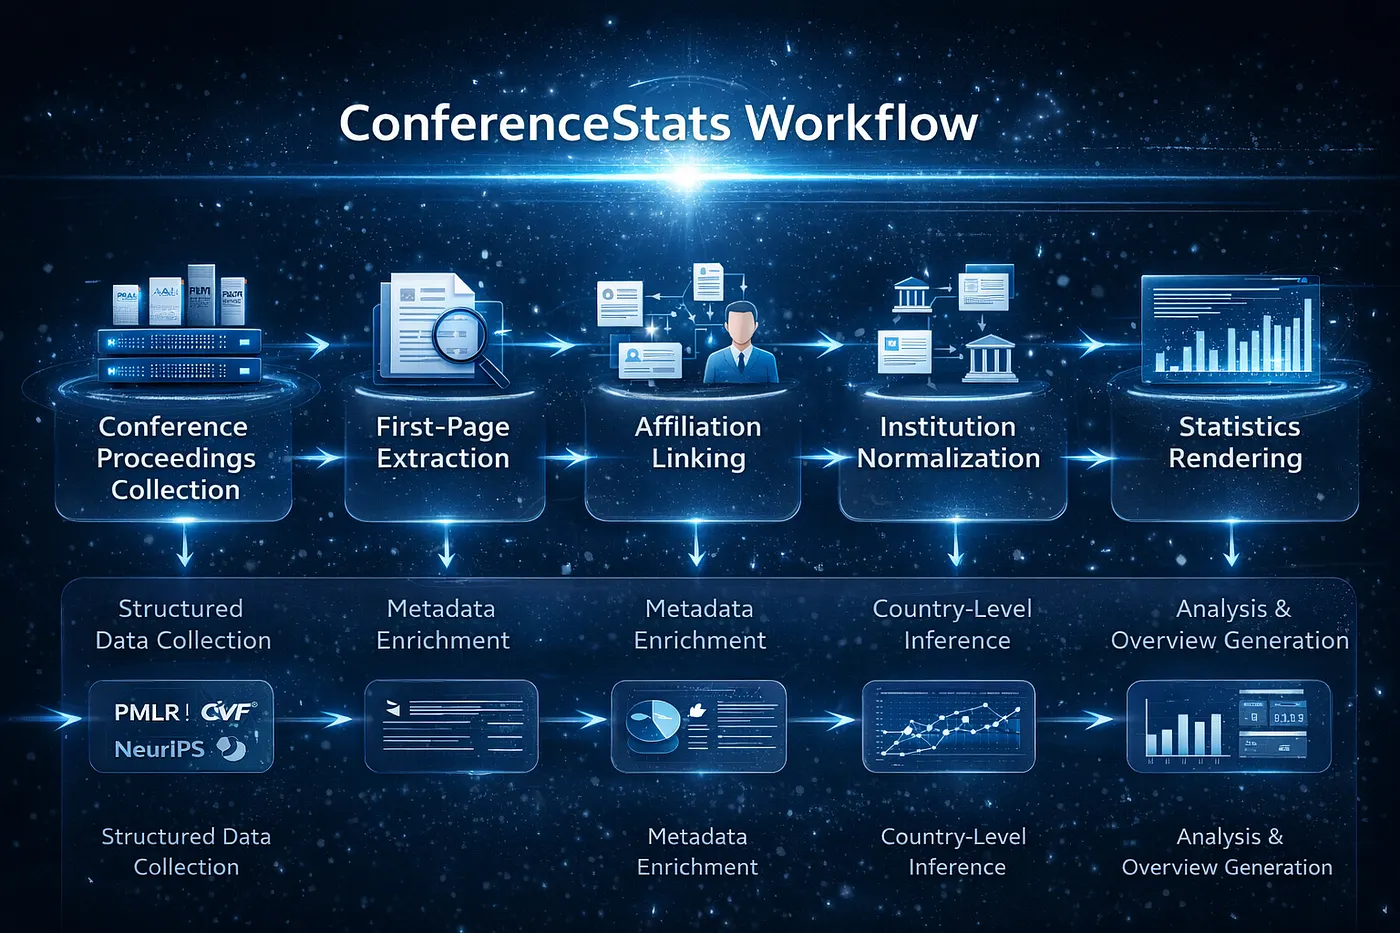
\includegraphics[height=.78\textheight]{img_13_03.png}
\end{center}
\end{frame}

\begin{frame}[t]{Fast alles ist jetzt einfach\dots}{Konferenzbeiträge aus China}
\begin{center}
  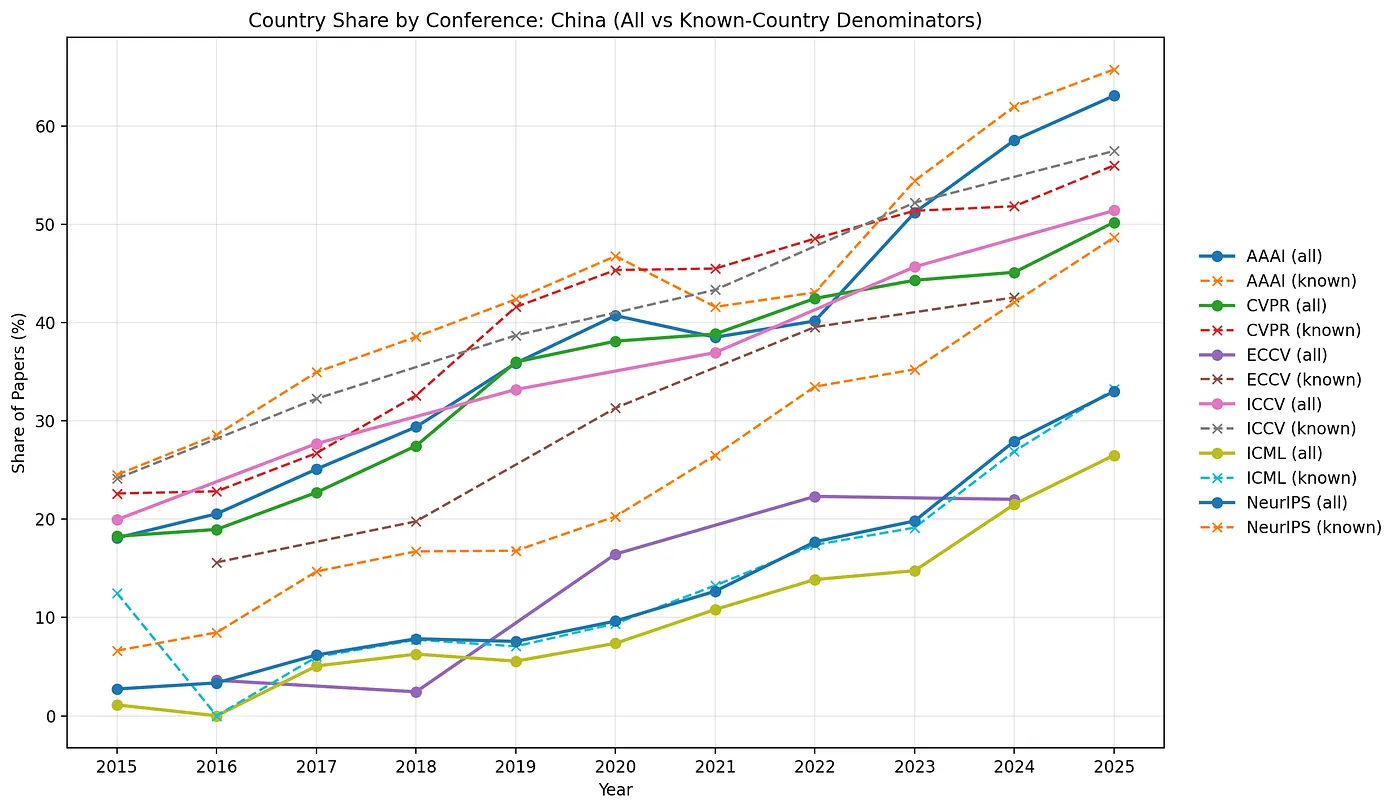
\includegraphics[height=.78\textheight]{img_13_04.png}
\end{center}
\end{frame}

% --------------------------------------------------------------------------
% Agent4CT - drei Folien aus dem Bangalore-Vortrag (india-talk), ins
% Deutsche übertragen für den MSD Senso-Abend.
% --------------------------------------------------------------------------
\begin{frame}[t]{Agent4CT}{Alle DL-CT-Methoden an einem Wochenende}
\begin{itemize}\itemsep=0.15em
  \item Kontinuierlich laufender LLM-Agent, der eine
        CT-Rekonstruktions-Codebasis bearbeitet, kurze GPU-Experimente
        ausführt und Änderungen nur dann übernimmt, wenn die Metriken
        es bestätigen. Fünf Agenten arbeiten parallel an fünf
        CT-Wettbewerben und tauschen Erkenntnisse über ein gemeinsames
        Scratchpad aus.
\end{itemize}
\vspace{0.3em}
\textbf{Nachimplementierte Solver}
({\small\ttfamily pentathlon/demo\_dl\_reference}):
\begin{columns}[T]
  \begin{column}{0.49\textwidth}
    \begin{itemize}\itemsep=0.1em\small
      \item \textbf{Analytisch:} PyroNN FBP (Syben 2019).
      \item \textbf{Klassisch-iterativ:} TV (iterativ, überwacht,
            Hyperparametersuche); Wu \emph{et~al.}\ 2015
            ($+$ trainierbarer Port).
      \item \textbf{Variational / unrolled:} Hammernik 2017
            Variational Network ($+$ CT-Port); Learned Primal-Dual
            (Adler \& \"Oktem); ITNet v1--v3.
      \item \textbf{Selbstüberwachtes Denoising:}
            Dual-Domain-U-Net und trainierbare bilaterale Filter
            (Wagner 2023 / 2022, mit überwachten Varianten).
    \end{itemize}
  \end{column}
  \begin{column}{0.49\textwidth}
    \begin{itemize}\itemsep=0.1em\small
      \item \textbf{Szenenbasierte neuronale Felder:} NAF
            (neural attenuation field); R2Gaussian.
      \item \textbf{Basismodelle:} RAM (Terris 2025).
      \item \textbf{Diffusions-Priors:} DDPM;
            Diffusions-Prior-Sampling; Diffusions-Rekonstruktion mit
            Datenkonsistenz.
      \item \textbf{Transformer:} U-Swin.
    \end{itemize}
  \end{column}
\end{columns}
\vspace{0.3em}
\begin{center}
  {\small\ttfamily github.com/akmaier/Agent4CT}
\end{center}
\end{frame}

\begin{frame}[t]{Agent4CT}{Vom Paper zum Benchmark}
\begin{itemize}\itemsep=0.25em
  \item \textbf{Enges Iterationsbudget.} 5~min pro GPU-Experiment
        zwingen den Agenten, Architektur gegen Durchsatz abzuwägen.
  \item \textbf{Zwischenkontrollen alle 30 Iterationen.}
        1~h Validierung auf einem $3\times$ größeren Subset erkennt
        Overfitting, bevor es sich ausbreitet.
  \item \textbf{Git-gestütztes Logbuch.} Jede übernommene Änderung
        ist ein Commit; verworfene Versuche entsprechen einem
        \texttt{git reset} plus einer Zeile in der Experiment-TSV.
  \item \textbf{Anti-Overfit-Regeln} werden in das
        \texttt{program.md} jedes Agenten übernommen -- so beginnt
        jeder neue Lauf auf den Schultern der anderen, nicht bei Null.
\end{itemize}
\end{frame}

\begin{frame}[t]{Agent4CT}{Das Pentathlon -- fünf CT-Bestenlisten}
\begin{columns}[T]
  \begin{column}{0.55\textwidth}
    \begin{itemize}\itemsep=0.2em
      \item AAPM 2016 Low-Dose-CT (Mayo)
      \item AAPM 2021 DL Sparse-View-CT (128-Sicht-Fächerstrahl)
      \item AAPM 2022 TrueCT
      \item AAPM 2022 DL-Spektral-CT
      \item AAPM 2024 CT-Metallartefaktreduktion
    \end{itemize}
    \vspace{0.4em}
    Bewertung: zurückgewonnenes \emph{Headroom} $\in [0,1]$;
    $1$ entspricht dem Orakel.
  \end{column}
  \begin{column}{0.45\textwidth}
    \centering
    \textbf{Aktuell bestes Ergebnis -- Brust-CT}\\[0.4em]
    Learned Primal-Dual\\
    SSIM $\mathbf{0{,}9062}$\\
    bei $1{,}49$\,Mio.\ Parametern
  \end{column}
\end{columns}
\end{frame}

% --------------------------------------------------------------------------
% Folie 15 - Basismodelle: Bayerisches KI-Basismodell
% --------------------------------------------------------------------------
\begin{frame}[t]{Basismodelle}{Bayerisches KI-Basismodell}
\begin{center}
  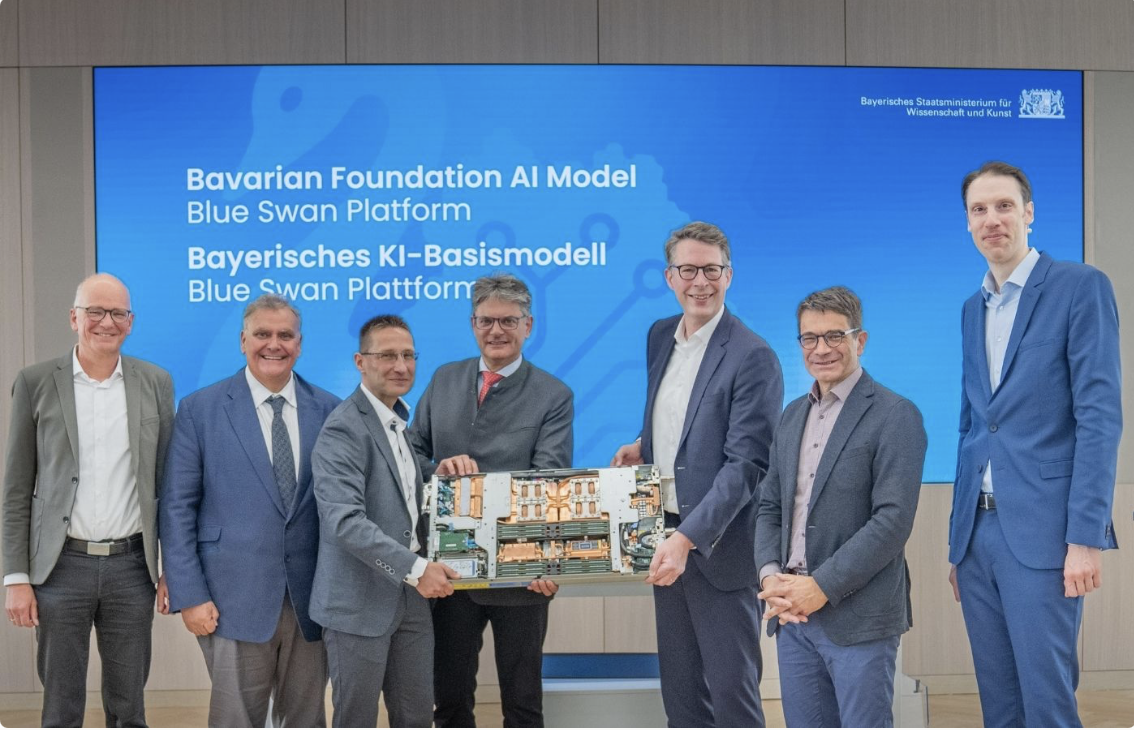
\includegraphics[height=.78\textheight]{img_14_01.png}
\end{center}
\end{frame}

% --------------------------------------------------------------------------
% Folien 15a-b - Neue Folien für MSD Senso-Abend: multimodale
% Basismodelle in der Onkologie am Beispiel PRAEGNANT
% --------------------------------------------------------------------------
\begin{frame}[t]{Basismodelle}{Multimodale Datenintegration in der Onkologie}
\vspace{0.2em}
Multimodale Basismodelle vereinen sehr unterschiedliche Datenquellen
in einem gemeinsamen Repräsentationsraum:
\vspace{0.4em}
\begin{columns}[T]
  \begin{column}{0.49\textwidth}
    \begin{itemize}\itemsep=0.15em\small
      \item \textbf{Multi-Omics:} Genom, Transkriptom, Proteom,
            Methylom.
      \item \textbf{Bildgebung:} CT, MRT, PET, Histopathologie,
            Mammographie.
      \item \textbf{Sprache:} Anamnese, Tumorboard-Mitschnitte,
            Arztbriefe.
    \end{itemize}
  \end{column}
  \begin{column}{0.49\textwidth}
    \begin{itemize}\itemsep=0.15em\small
      \item \textbf{Labordaten:} Blutwerte, Tumormarker,
            therapiebegleitende Verlaufsparameter.
      \item \textbf{LLMs:} Fachliteratur, Leitlinien,
            Studienprotokolle.
      \item \textbf{Simulationen:} Pharmakokinetik,
            Behandlungssimulationen, \emph{Digital Twins}.
    \end{itemize}
  \end{column}
\end{columns}
\vspace{0.6em}
\begin{center}\small
  $\Rightarrow$ Ein gemeinsames Modell anstelle vieler isolierter Werkzeuge.
\end{center}
\end{frame}

\begin{frame}[t]{Basismodelle}{Hypothesen aus Studiendaten -- PRAEGNANT}
\vspace{0.1em}
\begin{itemize}\itemsep=0.15em\small
  \item \textbf{PRAEGNANT}: deutsches akademisches Studiennetzwerk zum
        fortgeschrittenen Mammakarzinom (Fasching et~al.); Tumorgewebe,
        Blut, Biomarker und Patient-Reported Outcomes aus vielen
        Zentren und tausenden Patientinnen
        ({\ttfamily praegnant.org}).
\end{itemize}
\vspace{0.3em}
\begin{center}
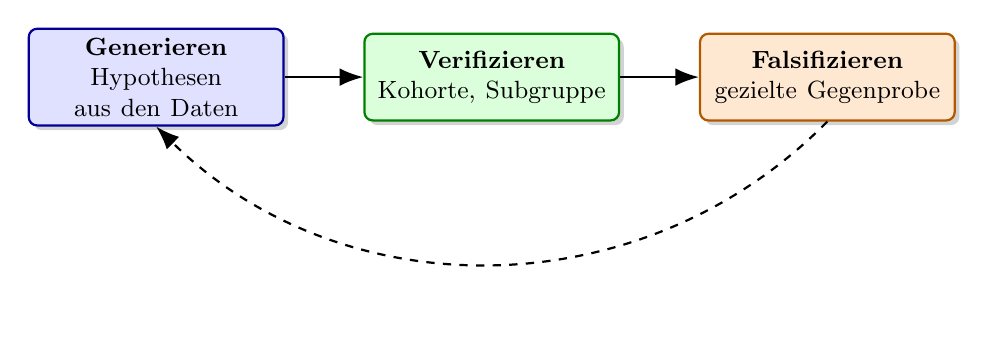
\begin{tikzpicture}[
    every node/.style={font=\small\bfseries},
    box/.style={draw, rounded corners=3pt, thick, minimum height=1.1cm,
                minimum width=3.2cm, text width=3.0cm, align=center,
                drop shadow={shadow xshift=0.6mm, shadow yshift=-0.6mm,
                             opacity=0.35}},
    gen/.style ={box, fill=blue!12,   draw=blue!60!black},
    ver/.style ={box, fill=green!14,  draw=green!50!black},
    fal/.style ={box, fill=orange!18, draw=orange!70!black},
    arr/.style ={-{Latex[length=3mm]}, thick}
  ]
  \node[gen]                    (g) {Generieren\\\small\mdseries Hypothesen aus den Daten};
  \node[ver, right=10mm of g]   (v) {Verifizieren\\\small\mdseries Kohorte, Subgruppe};
  \node[fal, right=10mm of v]   (f) {Falsifizieren\\\small\mdseries gezielte Gegenprobe};
  \draw[arr] (g) -- (v);
  \draw[arr] (v) -- (f);
  \draw[arr, dashed] (f.south) to[bend left=45] (g.south);
\end{tikzpicture}
\end{center}
\vspace{0.3em}
\begin{itemize}\itemsep=0.15em\small
  \item Das Basismodell schlägt aus den vereinheitlichten
        Multi-Omics-, Bildgebungs- und Klinikdaten \emph{neue
        Hypothesen} vor (z.\,B. Mutations-Therapie-Interaktionen,
        Bildmarker für das Therapieansprechen).
  \item \emph{Verifikation} per simulierter und retrospektiver
        Subgruppenanalyse in PRAEGNANT-ähnlichen Kohorten;
        \emph{Falsifikation} per gezielter Gegenprobe -- alles
        automatisch protokolliert und für Klinikerinnen und Kliniker
        nachvollziehbar.
  \item Ergebnis: vom Datensatz zu prüfbaren Studienhypothesen in
        Stunden statt Monaten.
\end{itemize}
\end{frame}

% --------------------------------------------------------------------------
% Folie 16 - Referenzen
% --------------------------------------------------------------------------
\begin{frame}[t]{Referenzen}
\scriptsize
\linespread{0.94}\selectfont
\begin{itemize}\itemsep=0.02em
  \item V.~Mnih, K.~Kavukcuoglu, D.~Silver, A.~Graves, I.~Antonoglou,
        D.~Wierstra und M.~Riedmiller,
        \emph{Playing Atari with Deep Reinforcement Learning},
        arXiv:1312.5602, 2013.
  \item D.~Silver et~al.,
        \emph{Mastering the game of Go with deep neural networks and tree search},
        \emph{Nature}, 529:484--489, 2016 (AlphaGo).
  \item K.~Hammernik, T.~Klatzer, E.~Kobler, M.~P.~Recht, D.~K.~Sodickson,
        T.~Pock und \textbf{F.~Knoll},
        \emph{Learning a Variational Network for Reconstruction of
        Accelerated MRI Data},
        \emph{Magnetic Resonance in Medicine}, 79(6):3055--3071, 2018
        (FastMRI / Variational Network).
  \item A.~Maier, C.~Syben, B.~Stimpel, T.~Wuerfl, M.~Hoffmann, F.~Schebesch,
        W.~Fu, L.~Mill, L.~Kling, S.~Christiansen,
        \emph{Learning with Known Operators Reduces Maximum Error Bounds},
        \emph{Nature Machine Intelligence}, 1:373--380, 2019.
  \item M.~Zaiss, J.~R.~Rajput, H.~N.~Dang, V.~Golkov, D.~Cremers,
        F.~Knoll und \textbf{A.~Maier},
        \emph{Exploring GPT-4 as MR sequence and reconstruction
        programming assistant: GPT4MR},
        BVM Workshop, S.~94--99, Springer, 2024.
  \item M.~Zaiss, A.~Aly, J.~Endres, T.~Dornstetter, S.~Weinmüller und
        \textbf{A.~Maier},
        \emph{Agentic MR sequence development: leveraging LLMs with MR
        skills for automatic physics-informed sequence development},
        arXiv:2604.13282, 2026 (Agent4MR).
  \item PRAEGNANT-Studie (metastasiertes Mammakarzinom):
        \url{https://praegnant.org}
  \item Deutscher Zukunftspreis (Niederfeld-MRT):
        \url{https://www.deutscher-zukunftspreis.de/de/die-gewinner-des-deutschen-zukunftspreises-2023-spendeten-ein-mrt-geraet}
  \item Bayerisches KI-Basismodell:
        \url{https://www.ai-bay.eu}
  \item Konferenz-Statistik-Werkzeug:
        \url{https://github.com/akmaier/ConferenceStats}
  \item Agent4CT -- agentische Nachimplementierung von
        Deep-Learning-CT-Methoden:
        \url{https://github.com/akmaier/Agent4CT}
\end{itemize}
\end{frame}

% --------------------------------------------------------------------------
% Folie 17 - Vielen Dank + QR-Code (zentriert, schwarz/weiß)
% --------------------------------------------------------------------------
\begin{frame}[t]{Vielen Dank!}
\begin{center}
  {\Large Folien auf GitHub}\\[1.2em]
  
\includegraphics[height=10cm]{qr_github.png}\\[0.8em]
  {\normalsize\ttfamily github.com/akmaier/AIMed2026Slides/tree/de-msd-senso}
\end{center}
\end{frame}

\end{document}
